% This document provides the style to be used for a MSc Thesis at the
% Parallel and Distributed Systems group
\documentclass[11pt,twoside,a4paper,openright]{report}

% math packages
\usepackage{amsmath}
\usepackage{amssymb}
\usepackage{makecell}
\usepackage{enumitem}
\usepackage{diagbox}
% textblocks for title page
\usepackage[absolute]{textpos}

% use babel for proper hyphenation
\usepackage[british]{babel}

% Graphics: different for pdflatex or dvi output, choose one
%\usepackage[dvips]{graphicx}
\usepackage[pdftex]{graphicx}
%\usepackage{graphicx}

\usepackage{epstopdf}
\usepackage{rotating}
\usepackage{subcaption}

% FONT
\usepackage[scaled=.92]{helvet}
%\usepackage{times}

% for url's use "\url{http://www.google.com/}"
\usepackage{url}
\usepackage[plainpages=false]{hyperref} 


% Information that will be filled in at various points in the report
\newcommand{\reportTitle}{Computational Imaging for Earth Surveillance}
\newcommand{\reportAuthor}{Pranav Sailesh Mani}
\newcommand{\reportEmail}{p.s.mani@student.tudelft.nl}
\newcommand{\reportUrlEmail}{\href{mailto:\reportEmail}{\reportEmail}}
\newcommand{\reportMSC}{Embedded Systems} %{Embedded Systems}{Computer Engineering}{Computer Science}{Electrical Engineering}
\newcommand{\reportDate}{\today} %TODO: Dit is de datum van uitgifte van final versie aan de afstudeer commissie 
\newcommand{\presentationDate}{\today} %TODO: Dit is de datum van de afstudeerpresentatie 
\newcommand{\graduationCommittee}{
Dr. ir. J.S.S.M. Wong & Computer Engineering, Delft University of Technology \\
Dr. ir. A.J. van Genderen & Computer Engineering, Delft University of Technology \\
Dr. ir. J.M. Kuiper & Aerospace Engineering, Delft University of Technology \\
Prof. dr. H.P. Urbach & Applied Sciences, Delft University of Technology \\
} % The order of listing the names: Graduation prof, supervisor(s), others ordered by title + alphabetical 
%examples: 
%prof. dr. ir. H. J. Sips (chair) & Delft University of Technology \\ 
%ir. dr. D. H. J. Epema           & Delft University of Technology \\ 
\newcommand{\reportAbstract}{TODO ABSTRACT}
\newcommand{\reportKeywords}{TODO KEYWORDS}

% For pdflatex
\pdfinfo{
   /Author (\reportAuthor)
   /Title  (\reportTitle)
   /Keywords (\reportKeywords)
}

\begin{document}

\pagenumbering{alph}
\pagestyle{empty}


% FRONTCOVER
\include{frontcover}

%%%%%%%%%%%%%%%%%%%%%%%%%%%%%%%%%%%%%%%%%%%%%%%%%%%%%%%%%%%%%%%%%%%%%%%%%%%%%%%
\hoffset=1.63cm
\oddsidemargin=0in
\evensidemargin=0in
\textwidth=5in

%%%%%%%%%%%%%%%%%%%%%%%%%%%%%%%%%%%%%%%%%%%%%%%%%%%%%%%%%%%%%%%%%%%%%%%%%%%%%%%
\parindent=1em

% EMPTY PAGE
\cleardoublepage

\pagestyle{plain}
\pagenumbering{roman}
\setcounter{page}{1}

% TITLE PAGE: page i (hidden)
\include{titlepage}

% GRADUATION DATA AND ABSTRACT: pages ii and iii (hidden)
%De aankondiging bevat de spreker, titel, plaats, datum en tijd, samenstelling van de afstudeercommissie en een korte samenvatting (maximaal 25 regels).
\thispagestyle{empty}

\noindent \textbf{Pranav Sailesh Mani}\\
\begin{tabular}{l}
\reportAuthor{} (\reportUrlEmail)\\
\end{tabular}\\
\noindent \textbf{Title}\\
\begin{tabular}{l}
\reportTitle\\
\end{tabular}\\
\noindent \textbf{MSc presentation}\\
\begin{tabular}{l}
% <MM> DD, YYYY (like \today)
30 November, 2017\\
\end{tabular}

\vspace{1.1cm}

\noindent \textbf{Graduation Committee}\\
\begin{tabular}{ll}
\graduationCommittee
\end{tabular}
\vspace{1.1cm}

\noindent \begin{tabular}{ll}
\textbf{Thesis Number - CE-MS-2017-14}
\end{tabular}

\begin{abstract} %de abstract bevat alleen een korte samenvatting van de inhoud van het onderzoek
\setcounter{page}{3}
\reportAbstract{ Cameras are used in various applications and one such common application has been space. Delfi Space is the CubeSat Development program of the Delft University of Technology and a subprogram of Defi-Space is Delfi-PQ which aims to develop PocketQubes which are an order of magnitude smaller than the CubeSat standards. One of the advanced payloads that would potentially be a part of the Delfi-PQ is an imager/camera. The imager needs to be as small as possible in order to fit into the Delfi-PQ satellites. The design of the camera has remained the same throughout the years and one of the reasons that increase the thickness of the camera is the presence of lenses. A way to reduce the size of the camera would be to remove the lens out of the equation. However, this introduces additional problems and trade-offs in the camera. These lenses can be replaced by masks/coded apertures. One of the additional steps in using coded-apertures is that additional computational steps need to be performed in order to reconstruct the image. The kind of computation that needs to be performed depends on the kind of masks that would be used. In this thesis, a separable mask is chosen and computer simulations on separable masks have been performed. Two image sensors that can be used in the picosatellite were chosen for implementation and the hardware/software is designed and developed. The experimental setup for determining the field of view of a lensless camera has been developed and tested. One of the trade-offs observed through the experiments is that the acceptance angle of a lensless imager had reduced by 38 percent and 31.8 percent in the horizontal and vertical directions compared to a conventional lens-based system. Based on the experimental results, the field of view of the camera has also been determined. A singular value decomposition based method has been developed and is used to align and calibrate the camera with the mask. The final step is estimating the system matrices of the lensless system. The system matrices enable the perfect reconstruction and a complete realization of a separable mask based lensless camera.  A scheme for estimating the system matrices of the lensless imager using Hadamard basis is proposed and confirmed using simulations and the strategy for experimental verification is proposed. As far as we know, this is the first study that focuses on designing and developing a lensless camera in the visible light domain for use in picosatellites. }
\end{abstract}

\clearpage

%\setcounter{page}{4}

% EMPTY PAGE: page iv
\cleardoublepage

% OPTIONAL QUOTATION: page v
%\include{quotation}
% EMPTY PAGE: page vi
%\cleardoublepage

% PREFACE: page v
\chapter*{Preface}
\addcontentsline{toc}{chapter}{Preface}
This document contains the work that I have been doing for the past eight months. These months just flew by and I enjoyed working in this multi-disciplinary project. Firstly, I am thankful to the almighty for providing me the strength to overcome various challenges I faced over the past two years of my master program which has been highly demanding. I have a long list of people whom I would like to thank and without whose support this project could not have been completed.
I would like to first thank my parents for providing me the financial support for coming to the Netherlands and doing my master studies at TU Delft. Without their encouragement and support, I would not be where I am now. Next, I would like to thank my master program co-ordinator and my supervisor, Arjan van Genderen who accepted to supervise me in this multi-disciplinary project. I would like to thank Delfi Space Program Manager, Mr. Jasper Bouwmeester, who first introduced me to my second supervisor Hans Kuiper. Hans provided me the support and was instrumental in understanding the requirements for designing the imager. Next, I would like to thank the Paul Urbach who introduced me to the Optica Research Group which is where I did all the experiments. I am extremely thankful to Phd students, Yifeng Shao and Sander Kojninberg. Yifeng was also my daily supervisor and helped me with understanding the theoretical physics, simulation of imaging algorithms and also on how to work with optical instruments. He continuously encouraged me to overcome challenges I faced along the way. I could not have asked for a better supervisor. I would also like to thank Sander for many discussions that very highly insightful and helped me to cross hurdles that I faced. On the whole, the Optica Research Group was a very nice place to work with very sociable people. Lastly, I would like to thank my friends in Delft for their support and encouragement. 


\noindent
Delft, The Netherlands

\noindent
\today

% EMPTY PAGE: page vi
\cleardoublepage

% TABLE OF CONTENTS: starting at page vii
\tableofcontents

\cleardoublepage

\pagenumbering{arabic}
\setcounter{page}{1}

% INTRODUCTION: page 1
\chapter{Introduction and Problem Statement}
\label{chp:introduction}
The history of cameras go back to 13th century when Aristotle first noticed how light passing through a small hole in a darkened room produced an image of the sun on the wall. 
Throughout the centuries, the basic design of cameras have been continuously changing with  different versions of the 'camera obscura'. 'Camera Obscura' is a phenomenon that occurs when when a scene is projected onto a pinhole and the image of that scene is formed on the surface opposite to that of a pinhole. 

In a pinhole camera, light passes through the pinhole and forms an image on the sensor/image plane.As the size of the pinhole increased, the quality of image formed on the plane decreased and as the pinhole size became smaller, lesser light was allowed which resulted in decreased field of view. With the development of science and due to the limitations of the pinhole, lenses were introduced to increase the size of the aperture, the sharpness of the image and the light throughput. As humanity progressed with the rapid pace in technology, we were able to capture images and store them on a film. With the digital explosion in early 1990s, the thin films were replaced by Charged Couple Devices(CCD). Then came the cameras based on Complementary Metal Oxide Semiconductors(CMOS). CCD and CMOS sensors reduced the size of cameras considerably and it was possible to develop low cost cameras in a large number. However, cameras have retained the lens throughout the years. Cameras are used for various applications and one such application is the space exploration domain. 

Delfi Space is the small satellite program of TU Delft that is mainly meant for education and technology demonstration in very small sized satellites. Delfi-PQ programme is a sub-programme of the Delfi Space programme that aims at developing extremely small but highly capable PocketQube satellites. PocketQubes are an order of magnitude smaller than the well known CubeSat standard which formed the basis of previous Delfi satellite projects. The dimensions of a PocketQube satellite would be 50mm * 50mm * 178mm and their volume would be approximately eight times smaller than CubeSats. One of the advanced payload that would be part of the Delfi-PQ would be an imager/camera that consumes extremely low power and would fit into the dimensions specified by the Delfi-PQ team. The thickness of the camera should be less than 6mm thick.
 
In order to reduce the size of a camera, it would be necessary to remove the lens from the camera as the thinnest lens based mobile camera is 5mm thick. The primary focus of a lens would be to focus light from distant objects onto the CMOS sensor. Light from distant objects reach the sensor even without the lens except that the light is incoherent and the CMOS sensor would not be able to form the object properly without a lens. However, the lens could also be replaced by coded apertures. Coded Apertures have been used in the late 20th century to image X-Ray sources of light. Lensless coded aperture cameras can be as small as $100 \mu m$ thick. By using lensless cameras, we could potentially reduce the form-facto multiple times to suit the requirements of Delfi-PQ. This thesis would address the following research question:


\textbf{Is it possible to design ``lensless coded" aperture cameras with a small form-factor(thickness $<$ 10mm) using COTS(commercial off-the-shelf) components that can be used in U-class Spacecrafts ?}
%However, the thesis would focus on the broader applications of lensless camera in satellites and would also make an attempt at addressing the camera satisfying the size requirements of the Delfi-PQ.

This question can be broken down into the following sub-questions:
\begin{itemize}
\item Would it be possible to design a lensless camera to capture astronomical objects in the visible range of light spectrum?
\item What would be the minimum possible form-factor that would be achievable and the effects of different factors such as diffraction effects, mask-to-sensor distance and reconstruction algorithms?
\item If possible, how would the lensless camera compare with the conventional lens based cameras used currently?
\item Would it be possible to design a lensless camera that would fit the size constraints of the Delfi-PQ?
\end{itemize}
\vspace{1\baselineskip}

\noindent




% CHAPTERS ... For instance: History/Prior Work, Design/Implementation, Experiments
\chapter{Literature Survey and Trade-off Analysis}
\label{chp:LitSurvey}
In this chapter, a state-of-the art study will be presented that could assist in design of the lensless imager with specifications mentioned in the previous chapter.
\section{Trade-off Analysis}
\label{sec:tradeOff}
\subsection{Camera Sensor}
The camera sensor is the core of the Delfi-PQ Imager. The performance of a camera is mainly limited by the image sensor that it uses\cite{cmos}. The camera sensor can be off two types namely, CCD(charge coupled device) or CMOS(Complimentary Metal Oxide Semiconductor). Both the types of CMOS sensors have their own advantages and disadvantages. TO understand the challenges that each type of sensor poses, we must understand how the sensors are designed.

The following factors have been chosen to  make a trade-off between the different CMOS sensors:
\begin{enumerate}
\item Resolution : When rating a camera, the first thing that comes to the mind is the resolution of the camera. The resolution of a camera is directly dependent on the number of pixels in the image sensor of the camera. 
\item Power Consumption : In the design of the PQ-Camera, the most important factor is the power consumption of the entire imager. The majority of the power consumption by the imager is dependent on the power consumption of the CMOS sensor. 
\item Availability : Even though there are innumerable number of CMOS sensors in the world, availability of CMOS sensors is quite low when it comes to small-scale. Many CMOS manufacturers require large scale orders.
\item Quantum Efficiency(QE) : Quantum Efficiency is the measure of efficiency of the camera sensor to convert incoming photons into electrons. The ratio of electrons generated during the digitization process to photons is called quantum efficiency.
\item Pixel Size : Pixel size is the size of each pixel unit in the CMOS camera. It is also an important factor considering that the signal produced by the CMOS sensor depends on the pixel size as well.
$$
Signal = Light Density * (Pixel Size)^2 * QE
$$
\item Electronic Interface : The electronic interface that can be used to retreive data from the CMOS sensor also plays an important role. Since the project uses a low-power microcontroller that has limited communication capabilities, it would be wise to chose an interface that is supported by the microcontroller. Recently available chips use LVDS/MIPI interface to send data. These interfaces are not supported by the microcontroller that is being used as an on-board computer.
\item Dynamic Range : Dynamic Range and SNR are used interchangeably in CMOS sensors. The only difference is that dynamic range considers only the temporal dark noise while SNR includes the root mean square of the shot noise as well.  
\item Shutter Type : Camera sensors use different types of shutters namely, global shutter and rolling shutter. Global shutter reduces the distortions due to fast moving artefacts while increasing the dark current. Rolling shutter has more distortions in the case of imaging moving artefacts, but also has lesser dark noise compared to global shutter. 
\item Voltage Level : Voltage level also has to be taken into account while choosing the sensor because if the CMOS sensor needs a voltage level higher than that of the main satellite bus voltage, then additional circuitry has to be introduced to step up the voltage level which in turn increases the overall system power.  
\item Operating Temperature : Operating temperature is an important factor to take into account when choosing an imaging sensor. Since the camera is going to operate in space, it is better if the CMOS sensor has a higher operating range of temperature. 
\item Overall Size and Weight : As the imager has to fit within specific dimensions, the overall size and weight of the CMOS sensor also needs to be taken into account.
\item Frame Rate: Even though, it is not required to have a camera sensor that is capable of high frame rates, it is an added advantage and higher frame rate camera could help in imaging larger areas of the earth if required. 
\item Price: While there are no specific cost constraints in the project, price has also been taken into account.
\end{enumerate}

\begin{table}[ht]
\caption{Comparison of Different Image Sensor Candidates}
\label{tbl:TradeoffCMOS}
\begin{tabular}{|c|c|c|c|c|c|c|c|c|c|c|}
\hline
\diaghead{\theadfont Diag ColumnmnHead II}%
{Factors}{Candidates}&
\thead{(a)}&\thead{(b)}&\thead{(c)}&\thead{(d)}&\thead{(e)}&\thead{(f)}&\thead{(g)}&\thead{(h)}&\thead{(i)}&\thead{(j)}\\
\hline
\textbf{Optical Parameters} & & & & & & & & & &\\
\hline
Resolution & & & & & & & & & & \\
\hline
QE & & & & & & & & & & \\
\hline
Pixel Size & & & & & & & & & & \\
\hline
Shutter type & & & & & & & & & & \\
\hline
Frame Rate & & & & & & & & & & \\
\hline
\textbf{\makecell{Electrical and \\other parameters}} & & & & & & & & & & \\
\hline
Power Consumption & & & & & & & & & & \\
\hline
Availability & & & & & & & & & & \\
\hline
Electronic Interface & & & & & & & & & & \\
\hline
DR and SNR & & & & & & & & & & \\
\hline
Voltage & & & & & & & & & & \\
\hline
Operating Temperature & & & & & & & & & & \\
\hline
Overall Size and Weight & & & & & & & & & & \\
\hline
Price & & & & & & & & & & \\
\hline
\textbf{Points} & & & & & & & & & & \\
\hline
\end{tabular}
\end{table}

\subsection{Compression Algorithms}

\subsection{Reconstruction Algorithms}


\chapter{Simulation of Reconstruction Algorithm}
This chapter will describe how the system can be mathematically modelled and how the mask for the lensless imager was designed. As mentioned in the previous chapter the system can be modelled as 
\begin{equation}
\label{eq:conv2}
y = \phi * x + e ;
\end{equation}
Ignoring the noise and converting the equation to fourier domain, the equation \ref{eq:conv2} can be re-written as
\begin{equation}
\label{eq:conv3}
F(y) = F(\phi)F(x)
\end{equation}
\begin{equation}
\label{eq:conv3}
F(x) = \frac{F(y)}{F(\phi)}
\end{equation}
\begin{equation}
\label{eq:conv4}
x = F^{-1}(\frac{F(y)}{F(\phi)})
\end{equation}
Equation \ref{eq:conv4} is the simplest possible computational inversion of the scene from the sensor. This method has also been used in \cite{Toeplitz}. As mentioned in the previous chapter, there are two types of masks that can be used for the purpose of encoding the scene onto the mask, namely separable and non-separable mask. MATLAB has been used for the purpose of simulating the algorithms. In this chapter, we would simulate two types of mask patterns, namely separable and non-separable mask patterns. A separable mask pattern is one in which the mask matrix $\phi$ can be expressed in-terms of two sub- matrices:
\begin{equation}
\phi = \phi_L * \phi_R
\end{equation}
Both $\phi_L$ and $\phi_R$ are doubly-toeplitz mask. The mathematical model is also changed as described by the equation \ref{eq:separable}. A non-separable mask is one which does not follow this property and follows equation \ref{eq:conv2}.

\section{Simulation of a non-separable mask}
The non-separable mask simulation was carried out as shown in Figure \ref{fig:non_sep_sim}.

\begin{figure}[ht]
\includegraphics[scale = 0.50]{pics/non_sep_sim_flow}
\caption{Simulation-Flow non-separable matrix}
\label{fig:non_sep_sim}
\end{figure}
\section{Simulation of a separable mask}
\chapter{Implementation}
In this chapter, we will be discuss about the implementation of hardware and software of the camera that would be used for subsequent experiments.
The main specifications of the chosen cameras are shown in Table \ref{tbl:camera_specs}. These specifications are taken from the sensor data sheet and the camera manual provided by the vendors of the camera\cite{OV2640Arducam}\cite{OV5642Arducam}\cite{OV2640DS}\cite{OV5642DS}.  
\begin{table}[]
\centering
\caption{ Key Specifications Specifications of sensors Chosen}
\label{tbl:camera_specs}
\begin{tabular}{|c|c|c|}
\hline
Specification & OV2640 &  OV5642 \\
\hline
Voltage Level & 3.3/5V &  3.3/5V\\
 \hline
Frame Buffer Size & 384 KB & 8MB \\
 \hline
 Active Pixel Array Size& 1600$\times$1200&  2592$\times$1944 \\
 \hline  
 Camera Dimensions & 34mm $\times$ 24mm & 34mm $\times$24mm\\
 \hline
 Sensor Dimensions & 5725 $\mu$m $\times$ 6285 $\mu$m& 6945 $\mu$m $\times$ 6695 $\mu$m\\
 \hline
 Pixel Size & 2.2 $\mu$m $\times$ 2.2 $\mu$m & 1.4$\mu$m $\times$ 1.4 $\mu$m\\
 \hline
 Weight & 20 grams & 20 grams \\
 \hline
 Operating Temperatures & -10 to 55 degree celsius & -10 to 55 degree celsius \\
 \hline
 Electronic Interfaces Needed & SPI, I2C & SPI, I2C\\
 \hline
 Dynamic Range & 50 dB & 68 dB \\
 \hline
\end{tabular}
\end{table}
\section{Embedded Software of Camera}
One of the main reasons behind choosing the OV2640 and OV5642 CMOS sensors is that they already have a ready electronic interface that can be used to interface with standard 8-bit/16-bit microcontrollers. Arducam is an open source camera that comes along with open-source hardware and software that is needed to capture images using the CMOS sensor. One of the core components in every camera made by Arducam is that there is a component called Arduchip\cite{Arduchip}. It is a basically an Altera MAXII CPLD EPM240 processor that facilitates DMA memory transfer between the camera memory module and components such as microcontroller and thereby helping to reduce the development time for special applications such as space where we the only computational resource that would be available are low power computing platforms such as microcontrollers with only synchronous serial interfaces such as I2C, SPI, etc. 

However, using the camera comes with its own advantages and disadvantages. The main advantage behind using this platform is that the platform has open-source libraries that could be used to interface with ATMEGA328P, an 8-bit microcontroller. In space-missions, it would not be possible to send high-powered microprocessors, and microcontroller is used as an on-board computer. Arducam has standard software libraries that can be used to interface with Arduino making the cumbersome and lengthy job of writing an interface software to a CMOS sensor way more easier.  A disadvantage of the hardware module is the on-board memory that it has to capture an image. The OV2640 Arducam mini camera module can capture upto $1600 \times 1200$ resolution images with or without any form of compression. However due to the limitation of the on-board OV2640 FIFO memory AL422B it would be possible to capture only compressed images and not full resolution RAW images. The AL422B on-board FIFO has only 384KB of memory and that is not enough to obtain a full-resolution RAW image. One of the other disadvantages is that custom code needs to be written to obtain various controls that we need for our camera. We have to write our own camera control software if we need to control factors such as exposure time, ISO, etc. as the default software uses automatic exposure control to enhance the image quality. The camera module architecture is shown in Figure \ref{fig:arducam_arch}. The OV5642 offers a greater flexibility in terms of memory as it has a larger FIFO Buffer(8 MB).

 \begin{figure}[!htbp]
\centering
\includegraphics[scale=0.75]{pics/arducam_architecture}
\caption{Camera Architecture of Arducam Mini OV2640 Camera Module}
\label{fig:arducam_arch}
\end{figure}

The system for experiments is as shown in Figure \ref{fig:imp_setup}. The Arduino is connected to the camera module through an I2C interface. Using the I2c interface it possible to set registers that control the functioning of the camera such as the output format, digital signal processing, etc. SPI interface is used to transfer the image data from the camera module to the Arduino. The Arduino upon receiving the image data either writes it to an  SD card or sends it to the software on the PC through the USB connection. The software flow is shown in Figure \ref{fig:arducam_software}. We use the same software flow for both the CMOS sensors as the APIs are designed for use with many sensor models. The same set of libraries can be used for different CMOS sensors by simply adding some preprocessor directives to a \texttt{memorysaver.h} header file provided in the open-source library. To see the images on the PC, the vendor has provided a host PC software(not-open source) and firmware which uses USB-UART to transfer images from the Arduino to PC. The firmware could be modified to ignore certain commands coming from the PC and using this we were able to modify the camera settings to our advantage. 
\begin{figure}[!htbp]
\centering
\includegraphics[scale=0.75]{pics/implementation_setup}
\caption{Implementation Setup}
\label{fig:imp_setup}
\end{figure}

One of the important factors that need to be controlled in camera is the exposure time. The Arducam libraries provide APIs for 10 different exposure levels for the OV5642 sensor. However, no such APIs are available for OV2640. Since OV2640 consumes lower power, it was decided to start the experiments with this camera. So, we need to write custom software to control the exposure level of this camera. The arducam APIs used for the software are shown in Table \ref{fig:arducam_software}. The details of more APIs can be found in the software application notes\cite{ArducamSoftwareApp}. The default camera settings were used with only modifications to exposure in the case of OV2640 module. The CMOS sensor can be directly accessed using \texttt{wrSensorReg16\_8, wrSensorReg8\_8} functions which provide I2C bus access to the CMOS sensor.
\begin{figure}[!htbp]
\centering
\includegraphics[scale  = 0.5]{pics/SoftwareFlowOV2640}
\caption{Software Flow used for image acquisition from CMOS sensors}
\label{fig:arducam_software}
\end{figure}


\begin{table}[]
\centering
\caption{ Details of Main APIs used}
\label{tbl:camera_apis}
\begin{tabular}{|c|c|c|}
\hline
API & Function \\
\hline
\texttt{InitCAM} & Initialize Camera Module\\
\hline
\texttt{set\_format} & \makecell{JPEG an BMP output formats \\can be selected}\\
\hline
\texttt{flush\_fifo} &  \\
\texttt{clear\_fifo\_flag} & \makecell{These functions are used to control \\the FIFO buffer, \\read the size of \\the image  and \\to reset them when needed}  \\
\texttt{read\_fifo\_length} & \\ 
\texttt{set\_fifo\_burst} & \\ 
\hline
\texttt{write\_reg} & \makecell{This function is used to write \\values to the specified register\\ address on the Arduchip.}\\
\hline
\texttt{wrSensorReg16\_8, wrSensorReg8\_8} & \makecell{These functions are used set camera \\ registers using I2C. The first function \\ is used for 16-bit register addresses and the \\second function is used for 8-bit addresses}  \\
\hline
\texttt{OV2640\_set\_JPEG\_size} & \makecell{These functions are used \\to set the resolution of the output image } \\
\texttt{OV5642\_set\_JPEG\_size} & \\
\hline
\texttt{OV5642\_set\_Exposure\_level} & \makecell{This functions are used \\to set the exposure level of the \\OV5642 CMOS sensor}\\
\hline
\end{tabular}
\end{table}
\subsection{Exposure Control of OV2640}
In order to do experiments, it was required to control the exposure of the camera. In the default driver that was provided by the vendor, the exposure was automatically set using the Automatic Exposure Control (AEC) feature in the sensor. So, a modification was needed in the driver software. Fortunately, the driver is open source and the there were libraries that could assist in setting the on-board registers through the I2C interface on the Arduino. First, let us have a look at how exposure control works in an OV2640 camera. All rolling shutter image sensors including OV2640 exposure the sensor one-line at a time i.e. pixels in the same line are exposed at the same time and different pixels in different lines are exposed at a different time. So, the minimum exposure time would be one line time and the maximum exposure time would be the frame time. This is illustrated in Figure \ref{fig:RollingShutterOV2640}. By default the pixel clock is set at 36MHz. We can calculate the minimum line time using the following equation:

$$
Minimum Exposure Time = 1/Pixel Clock * Pixel Clockes per line 
$$
As shown in Figure \ref{fig:ShutterTimingOV2640}, one line consists of 1922 pixel clocks(1600 for pixel data and 322 clocks of horizontal blanking). So the minimum exposure time would be 53.39$\mu$seconds and the maximum exposure time would be the frame time(multiply line time by 1200 + 44 lines of vertical blanking) which would be 66.63ms\cite{RollingShutterOV2640}. In order to control the exposure of the camera it is necessary to modify registers of address 4, 10, 13, 45. So, these registers were modified according the the required exposure time value. The driver software on the Arduino was modified to obtain different exposure times.
\begin{figure}[ht]
\includegraphics[width=\textwidth]{pics/rolling_shutter}
\caption{Rolling Shutter Operation on OV2640\cite{RollingShutterOV2640}}
\label{fig:RollingShutterOV2640}
\end{figure}

\begin{figure}[ht]
\includegraphics[width=\textwidth]{pics/OV2640timing}
\caption{Shutter Timing Diagram of OV2640\cite{RollingShutterOV2640}}
\label{fig:ShutterTimingOV2640}
\end{figure}

    \begin{figure}[ht]
    \centering
    \begin{subfigure}{0.5\textwidth}
    \centering
        \includegraphics[width=0.5\linewidth]{pics/exposure/60us}
        \caption{60 $\mu$seconds}
        \label{fig:exp60us}
    \end{subfigure}%
    \begin{subfigure}{0.5\textwidth}
    \centering
        \includegraphics[width=0.5\linewidth]{pics/exposure/1ms}
        \caption{1ms}
        \label{fig:exp1ms}
    \end{subfigure}
    
    \begin{subfigure}{0.5\textwidth}
    \centering
        \includegraphics[width=0.5\linewidth]{pics/exposure/5ms}
        \caption{5ms}
        \label{fig:exp5ms}
    \end{subfigure}%
    \begin{subfigure}{0.5\textwidth}
    \centering
        \includegraphics[width=0.5\linewidth]{pics/exposure/10ms}
        \caption{10ms}
        \label{fig:exp10ms}
    \end{subfigure}
        
        \begin{subfigure}{0.5\textwidth}
    \centering
        \includegraphics[width=0.5\linewidth]{pics/exposure/20ms}
        \caption{20ms}
        \label{fig:exp20ms}
    \end{subfigure}%
    \begin{subfigure}{0.5\textwidth}
    \centering
        \includegraphics[width=0.5\linewidth]{pics/exposure/60ms}
        \caption{60ms}
        \label{fig:exp60ms}
        
    \end{subfigure}    
    \caption{Images of a laser beam caught in different exposure times(with lens)}
    \label{fig:exptests}
    \end{figure}
    
\section{Power Consumption of Sensors}
 One important aspect that also needs to be taken into account is the power consumption of the camera module(including the sensor, memory, voltage regulators, etc). Since, we have two camera modules, OV2640(low resolution, low power) and OV5642(high resolution, high power). The power consumption profile for OV2640 was provided by the manufacturer, however, the same is not available for OV5642. So, it was decided to perform power consumption measurements for the sensors manually. In order to find the amount of power consumed, we connect a 1 $\omega$ resistor in series with the power line connecting the microcontroller and CMOS image sensor. The voltage measured across the resistor would be the current consumed by the camera sensors. The camera was operated in two modes: one in continuous "on" mode and the second mode was "on only when use". The second mode was activated clearing \texttt{GPIO\_PWDN\_MASK} when the camera is in use and setting it once again once the camera is done taking the pictures and then saving it onto the memory card. The current consumption graph is shown in Figure \ref{fig:power}.
 
   \begin{figure}[ht]
    \centering
    \begin{subfigure}{\textwidth}
    \centering
        \includegraphics[width=1\linewidth]{pics/power_1.JPG}
        \caption{Voltage across  resistor when continuosly on}
    \end{subfigure}%
   
    \begin{subfigure}{\textwidth}
    \centering
        \includegraphics[width=1\linewidth]{pics/power_2.JPG}
        \caption{Voltage across  resistor when  using \texttt{GPIO\_PWDN\_MASK}}
    \end{subfigure}
       \caption{This figure shows the difference between keeping the OV5642 sensor module continuously on and using the \texttt{GPIO\_PWDN\_MASK}}
        \label{fig:power}
   \end{figure}
 
 It can be seen from Figure \ref{fig:power} that we can reduce power consumption by switching on the camera only when in use. The camera is operated in 5V mode. The current consumed by the camera is averaged  and the measured power consumption is shown in Table \ref{tbl:power_cons}. As expected, the higher resolution camera OV5642 consumes more power than OV2640. Since, OV2640 is consumes lower power and is also of lower resolution(which implies lesser size), we proceed to continue with the next set of experiments using OV2640.
\begin{table}[]
\centering
\caption{measured power consumption of Cameras only when "on"}
\label{tbl:power_cons}
\begin{tabular}{|c|c|}
\hline
Sensor & Power \\
\hline
 OV2640 & 5V/93mA\\
 \hline
 OV5642 & 5V/233mA\\
 \hline
\end{tabular}
\end{table}
\chapter{Experiment to determine Acceptance Angle of CMOS sensor}
\label{chp:Experiment_FOV}
In this chapter, we will be discussing the experimental approach to finding the acceptance angle or the acceptance cone of the CMOS sensor. The acceptance cone primarily determines the field of view of the lensless imaging system. In the absence of lenses, the acceptance angle of the imaging sensor is determined by the acceptance angle of the micro-lens array on the surface of the image sensor. Hence, it is extremely important to determine the acceptance angle through an experimental approach. From this chapter onwards, all the experiments described are performed without the use of any lenses in front of the image sensors. Also, it must be noted that the terms CMOS sensor and image sensor are used in the place of each other and they both mean the same thing in our case.
\section{Testing of Acceptance Cone of Sensor}
\subsection{Experimental Setup}
A study conducted previously\cite{cra2} has employed cat's eye reflectometer method using four spherical lenses to accurately measure the chief ray angle of a CMOS sensor up to 0.65$\degree$\cite{cra2}. Apart from this, Armstrong Optical uses another complex method for measuring the chief ray angle or the acceptance angle\cite{cra1}. However, our work employs a simpler method to measure the acceptance cone of a CMOS sensor without the use of any lenses. Our method uses a collimated laser beam(650 nm), a pinhole for finding the accurate center of the axis and a rotational stage(to measure angular rotation) to find the response of the sensor to light at different angles and in-turn the acceptance cone of the sensor. 
Figure \ref{fig:exp_acc} shows the experimental setup that was made to measure the acceptance cone of the sensor. A collimated laser beam was reflected off a mirror and it is passed through a pinhole. The pinhole is mainly used to align the sensor with the beam. The pinhole produces a diffraction pattern that can be used to align the image sensor with the center of the beam. The difference in measurements with and without pinhole is shown in Figure \ref{fig:pinholeDiff}.
 \begin{figure}[ht]
\centering
\includegraphics[scale=0.50]{pics/acceptanceCone.png}
\caption{Experimental Setup for detection of acceptance cone}
\label{fig:exp_acc}
\end{figure}

\begin{figure}[ht]
    \centering
    \begin{subfigure}{0.5\textwidth}
    \centering
        \includegraphics[width=0.5\linewidth]{pics/withoutPinhole.jpg}
        \caption{Image without pinhole}
        \label{fig:nopinhole}
    \end{subfigure}%
    \begin{subfigure}{0.5\textwidth}
    \centering
        \includegraphics[width=0.5\linewidth]{pics/withPinhole.jpg}
        \caption{Image with pinhole}
        \label{fig:pinhole}
    \end{subfigure}
    \caption{Images of a laser beam caught with and without pinhole}
    \label{fig:pinholeDiff}
    \end{figure}
The pinhole cannot be used to measure the acceptance cone of the sensor because the waveform from the pinhole is a linear combination of different plane waves from different angles. Hence, this measurement was done without a pinhole. In order to measure the acceptance cone of the sensor, it is necessary to identify a portion of the image that can be taken as a reference to plot the variation in the signal measurement. It was assumed that the maximum point in the image can be taken as the signal. Since there was too much variation in the intensities measured, it was decided that we would average the 10 images in each angular position to reduce the signal noise. The maximum value in the image was taken and normalized and the measurements were repeated from -45$\degree$ to +45$\degree$ for 10 sets. The data from the red channel is analyzed. The exposure value was chosen such that the output does not saturate(does not reach 255) for any value in the image(See Figure \ref{fig:exp_acc_exp}). The maximum value in the image versus the angle is plotted. The ideal exposure value would be the one in which the signal does not saturate and there is still some room for additional signals. This is also indicated in Figure \ref{fig:exp_acc_exp}.
\begin{figure}[ht]
\centering
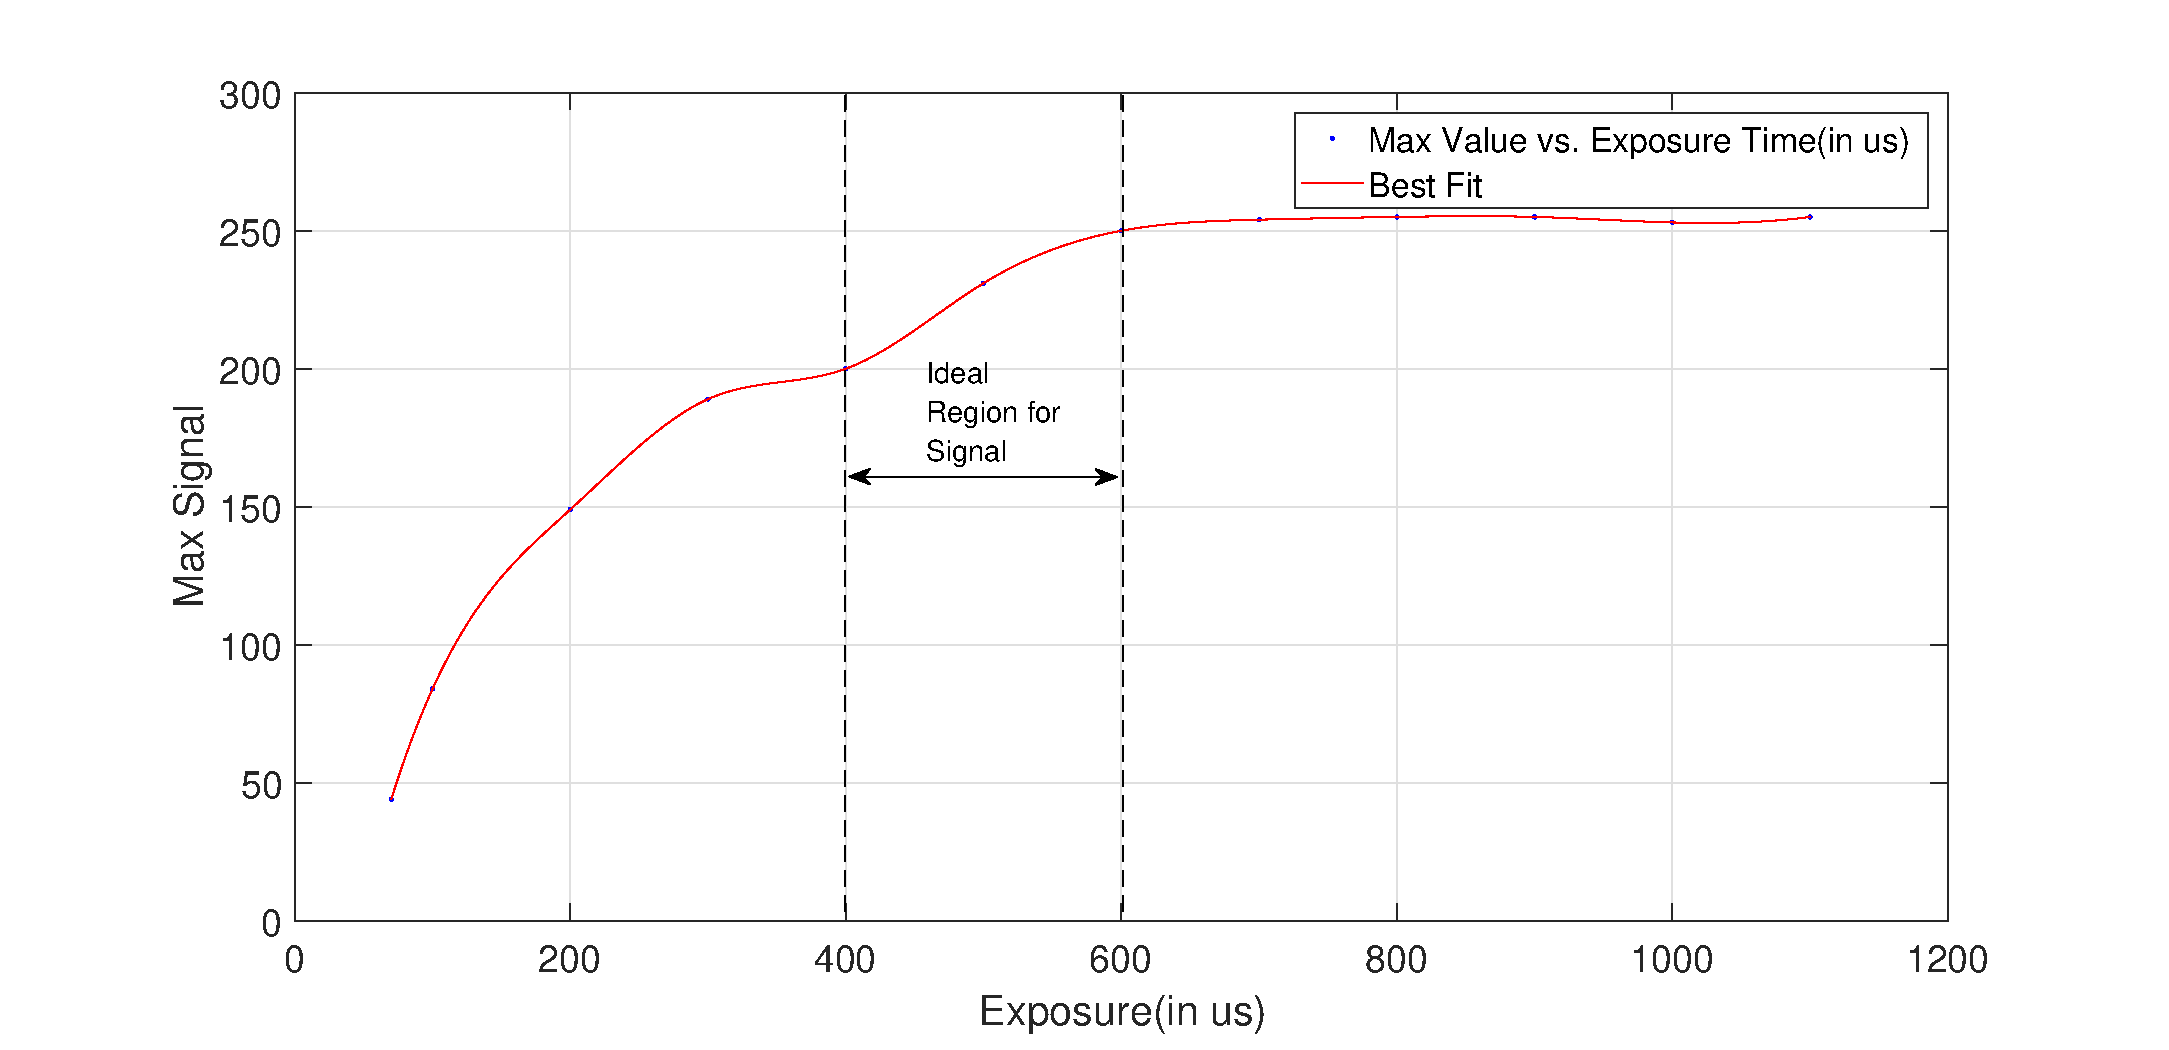
\includegraphics[width = \textwidth]{pics/ExposureTests}
\caption{Response for different Exposure values in microseconds}
\label{fig:exp_acc_exp}
\end{figure}

The obtained response curve for red channel is shown in Figure \ref{fig:exp_acc_red_1}. The normalized signal values are plotted with the standard deviation obtained for each angle are indicated with the use of an error bar. The best obtained curve fit is also plotted.
 \begin{figure}[ht]
\centering
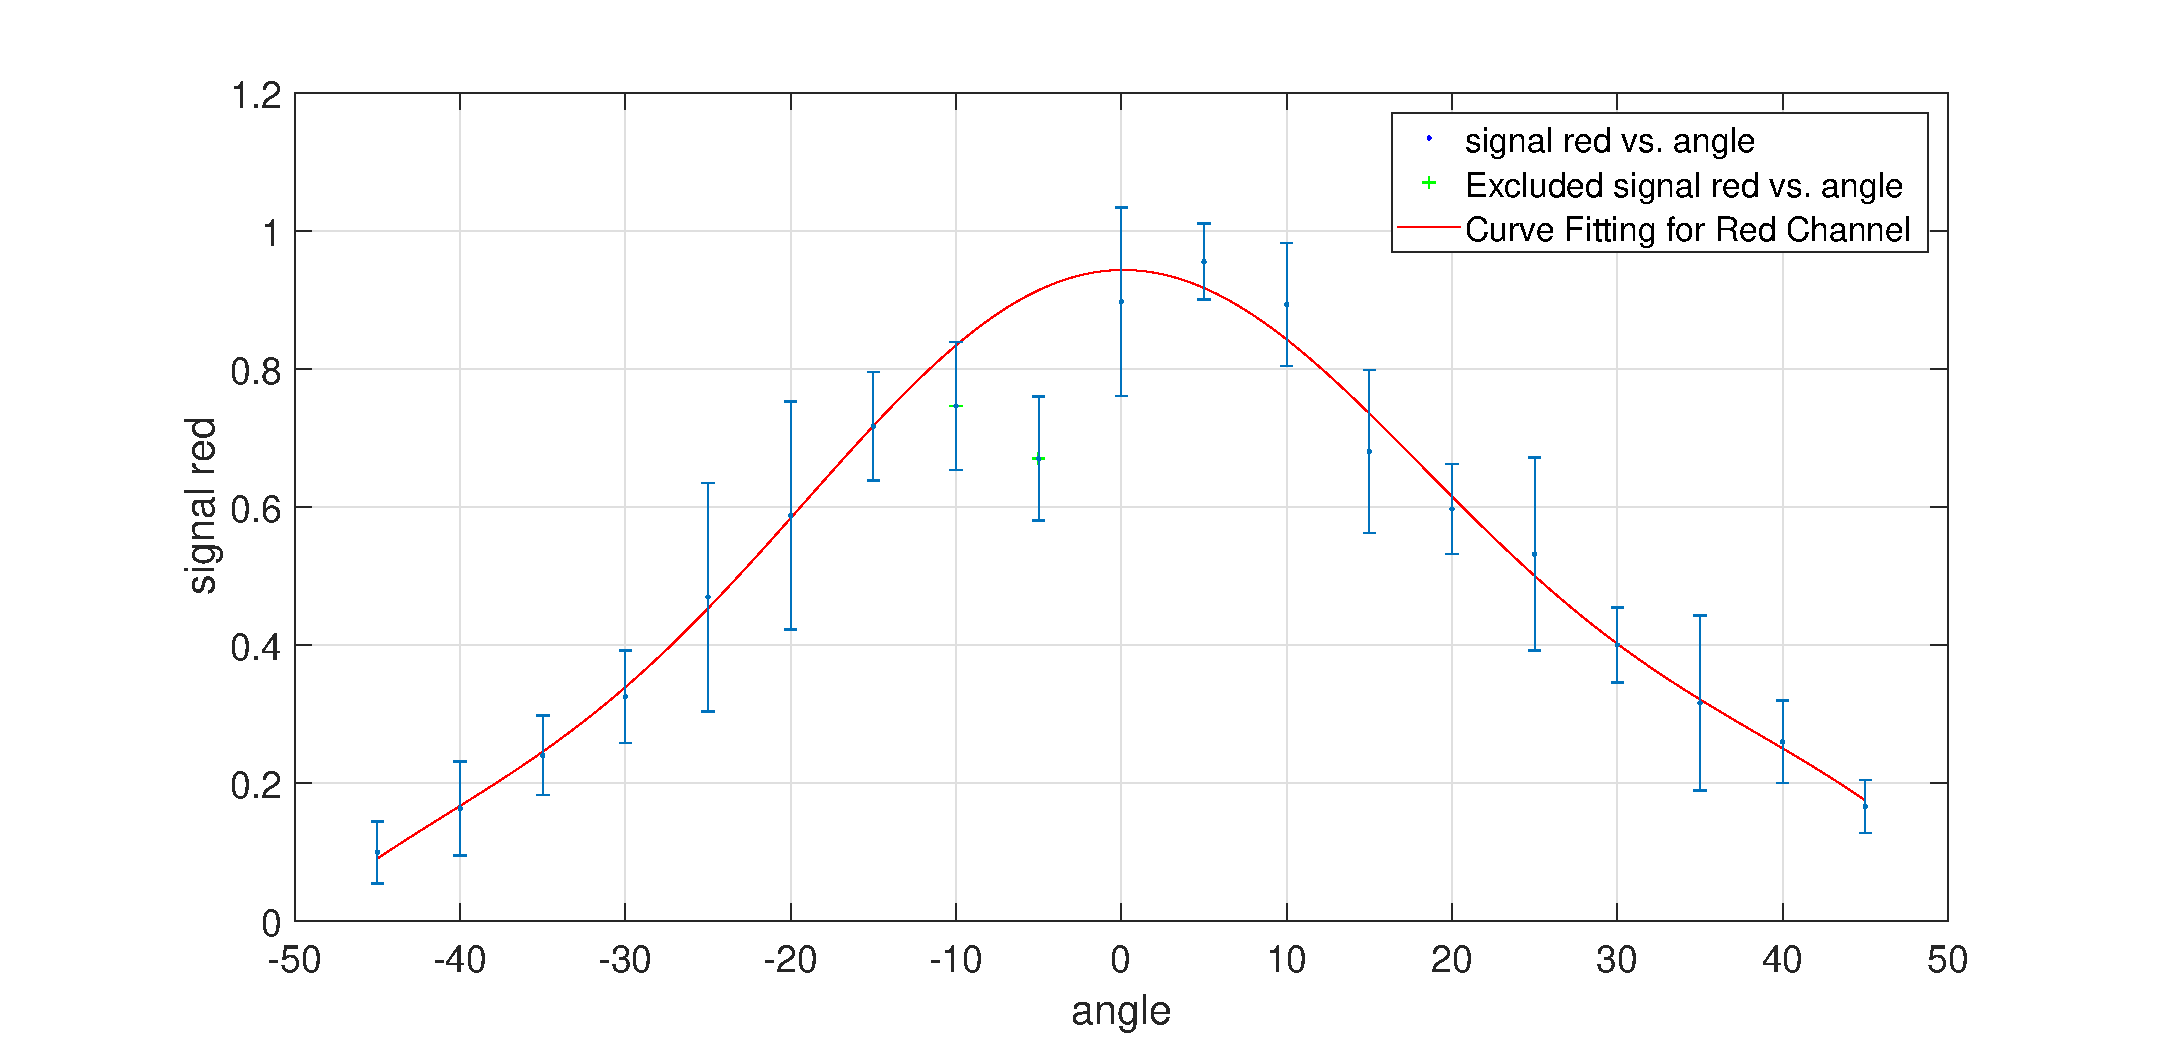
\includegraphics[width = \textwidth]{pics/RedChannel}
\caption{Response for Red Channel in Initial Experiment}
\label{fig:exp_acc_red_1}
\end{figure}

The initial observations from the results obtained are:
\begin{itemize}
\item There seems to be a very large standard deviation for each angle.
\item There seems to very sharp outliers at -5$\degree$ and -10$\degree$ which is a highly unexpected behavior.
\end{itemize}
These two observations point to experimental error. The error in the experimental results could be due to the following reasons:
\begin{itemize}
\item \textbf{Error introduced due to the translation of the rotational stage :} In order to make sure that the beam always hits the stage is translated if the beam does not hit due to the translation of the sensor away from the beam. This introduces an additional angular error which is not taken into account in the initial experiment. So, the stage was calibrated using the pinhole. If the sensor is exactly at the center of rotation of the rotational stage, the laser beam must always hit the same position of the sensor no matter what the rotational angle may be. The position of the sensor on the rotational stage was calibrated such that the signal(image with pinhole) obtained always remained at the center of the sensor. 

\item \textbf{Improper Reference Signal from Image :} At times, it was observed that the maximum point in the image occurs at different and unexpected points that are outside the beam. This also leads to different parts of the signal being measured each time. The outliers in the results could also mean that. An example average image in which the maximum is obtained at the end of the beam is shown in Figure \ref{fig:exp_acc_improper}. The point from where the signal is obtained is marked using a yellow star in the Figure \ref{fig:exp_acc_improper}.
\begin{figure}[ht]
\centering
\includegraphics[width = 0.75\textwidth]{pics/ImproperDetection}
\caption{Improper Reference Point for Signal}
\label{fig:exp_acc_improper}
\end{figure}
\item \textbf{Large Variation in the intensity of output image :} It was noticed that there was a huge variation in intensity for subsequent measurements at the very subsequent instants. This variation in the output is the cause of the large standard deviation in the result. Initially, I thought that this could be due to a relatively low exposure time(as lower exposure could lead to more output noise) or due to the variation of intensity of laser beam. Increasing the exposure time did give lower variations but the problem was traced to the automatic gain control(AGC) in the OV2640 image sensor. The amplifier gain of each pixel was adjusted automatically and this led to different intensities in subsequent readings. After this feature was turned off by modifying the driver software using I2C, it seemed that the variation in the output was no longer there.

\item \textbf{Unexpected Colors in the output image :} An unexpected feature in the image is seen in each measurement. The unexpected feature is the presence of green and blue colors of the laser beam. Since the laser beam is red with an almost constant wavelength in the red visible light region, the output of green is unexpected. This was very strange and upon studying the sensor, it seemed that the sensor had an automatic white balance(AWB) feature of OV2640. This white balance feature assumes a ``gray" world(wherein the average of all colors in the world is gray)\cite{OV2640SoftwareApp} which is not true in our case. The difference in the output is with and without AWB is shown in Figure \ref{fig:AWB}. Even after this adjustment, there seems to be a slight tinge of green at negative angles where the beam seems to ``dim" out. Even after trying out a variety of different settings this green could not be eliminated and could be due to Black Level Calibration in the sensor. The function of Black Level Calibration (BLC) is to produce accurate color in the dark area of the picture. There is no mention of how to turn off this feature in the datasheet or the application notes of this sensor. The vendor of the camera did not provide any information on how to turn off this feature. Hence, it was assumed that the sensor does not make any modifications to the red channel in angles where the signal ``dims" out.
\begin{figure}[ht]
    \begin{subfigure}{0.5\textwidth}
    \centering
        \includegraphics[width=0.5\linewidth]{pics/awb.jpg}
        \caption{Image with AWB}
    \end{subfigure}%
    \begin{subfigure}{0.5\textwidth}
    \centering
        \includegraphics[width=0.5\linewidth]{pics/withoutawb.jpg}
        \caption{Image without AWB}
    \end{subfigure}
    \caption{Images of a laser beam caught with and without pinhole}
    \label{fig:AWB}
    \end{figure}
\end{itemize}
\subsection{Improved experiment}
As mentioned in the previous experiment, the stage was calibrated such that the sensor remains at the center of rotation of the rotational stage. The reference signal was chosen such that the same point of the beam is always measured. In order to make sure that the same point of the beam is measured with and without pinhole, the coordinate of the central diffraction pattern is stored for different angular positions for -45$\degree$ to +45$\degree$ and the reference signal is taken from this point. In order to detect the central region in the output, a function called \texttt{imfindcircles} is used\cite{imfindcircles}. This function finds circles in an image using circular Hough transform. The readings for a specific angle are averaged and a logarithmic function is applied which is then passed to the \texttt{imfindcircles} function to detect the brightest possible circle with a radius of 3 pixels(This value was tuned such that the central portion is detected with 100 percent accuracy). The detection process using this method provided 100 percent accuracy for detection of the center of the central fringe pattern coordinate. This is illustrated in Figure \ref{fig:center_calib}. The Automatic gain controls and Automatic White balance features of the CMOS sensors were turned off by using suitable register settings mentioned in \cite{OV2640DS}. The Arduino was programmed to set the register values using I2C. The exposure was set at 500$\mu$s based on the exposure graph(See Figure \ref{fig:exp_acc_exp}).
\begin{figure}[!h]
\centering
\includegraphics[scale=0.300]{pics/CentralRegionTracking.jpg}
\caption{Coordinate Detection for central region signal detection}
\label{fig:center_calib}
\end{figure}

In the first step of the experiment, the rotational stage is rotated from -45$\degree$ to +45$\degree$ with pinhole and the coordinates of the central diffraction pattern is stored in a variable. In the second step of the experiment, the pinhole is removed and the signal is taken for different angles from the center coordinates measured using the diffraction pattern. This will ensure that we measure the same part of the beam every time we take a signal for measurement. After this, the signal is taken with a different offset(from the central diffraction pattern) in the X-direction to make sure that all the pixels behave in the same manner. The graphs for 100 different pixel positions in X-direction from the central position is shown in Figure \ref{fig:offset_calib}. From this graph, it can be seen that all the pixels in the same line exhibit the same behavior with a slight shift in angular position peak. In figure \ref{fig:offset_calibY}, the response for different pixels in the Y-direction is shown. It can be seen that there is a wider variation in the curve peak position. It can also be seen that all the pixels follow the same pattern with a slight shift in the peaks.
\begin{figure}[!h]
\centering
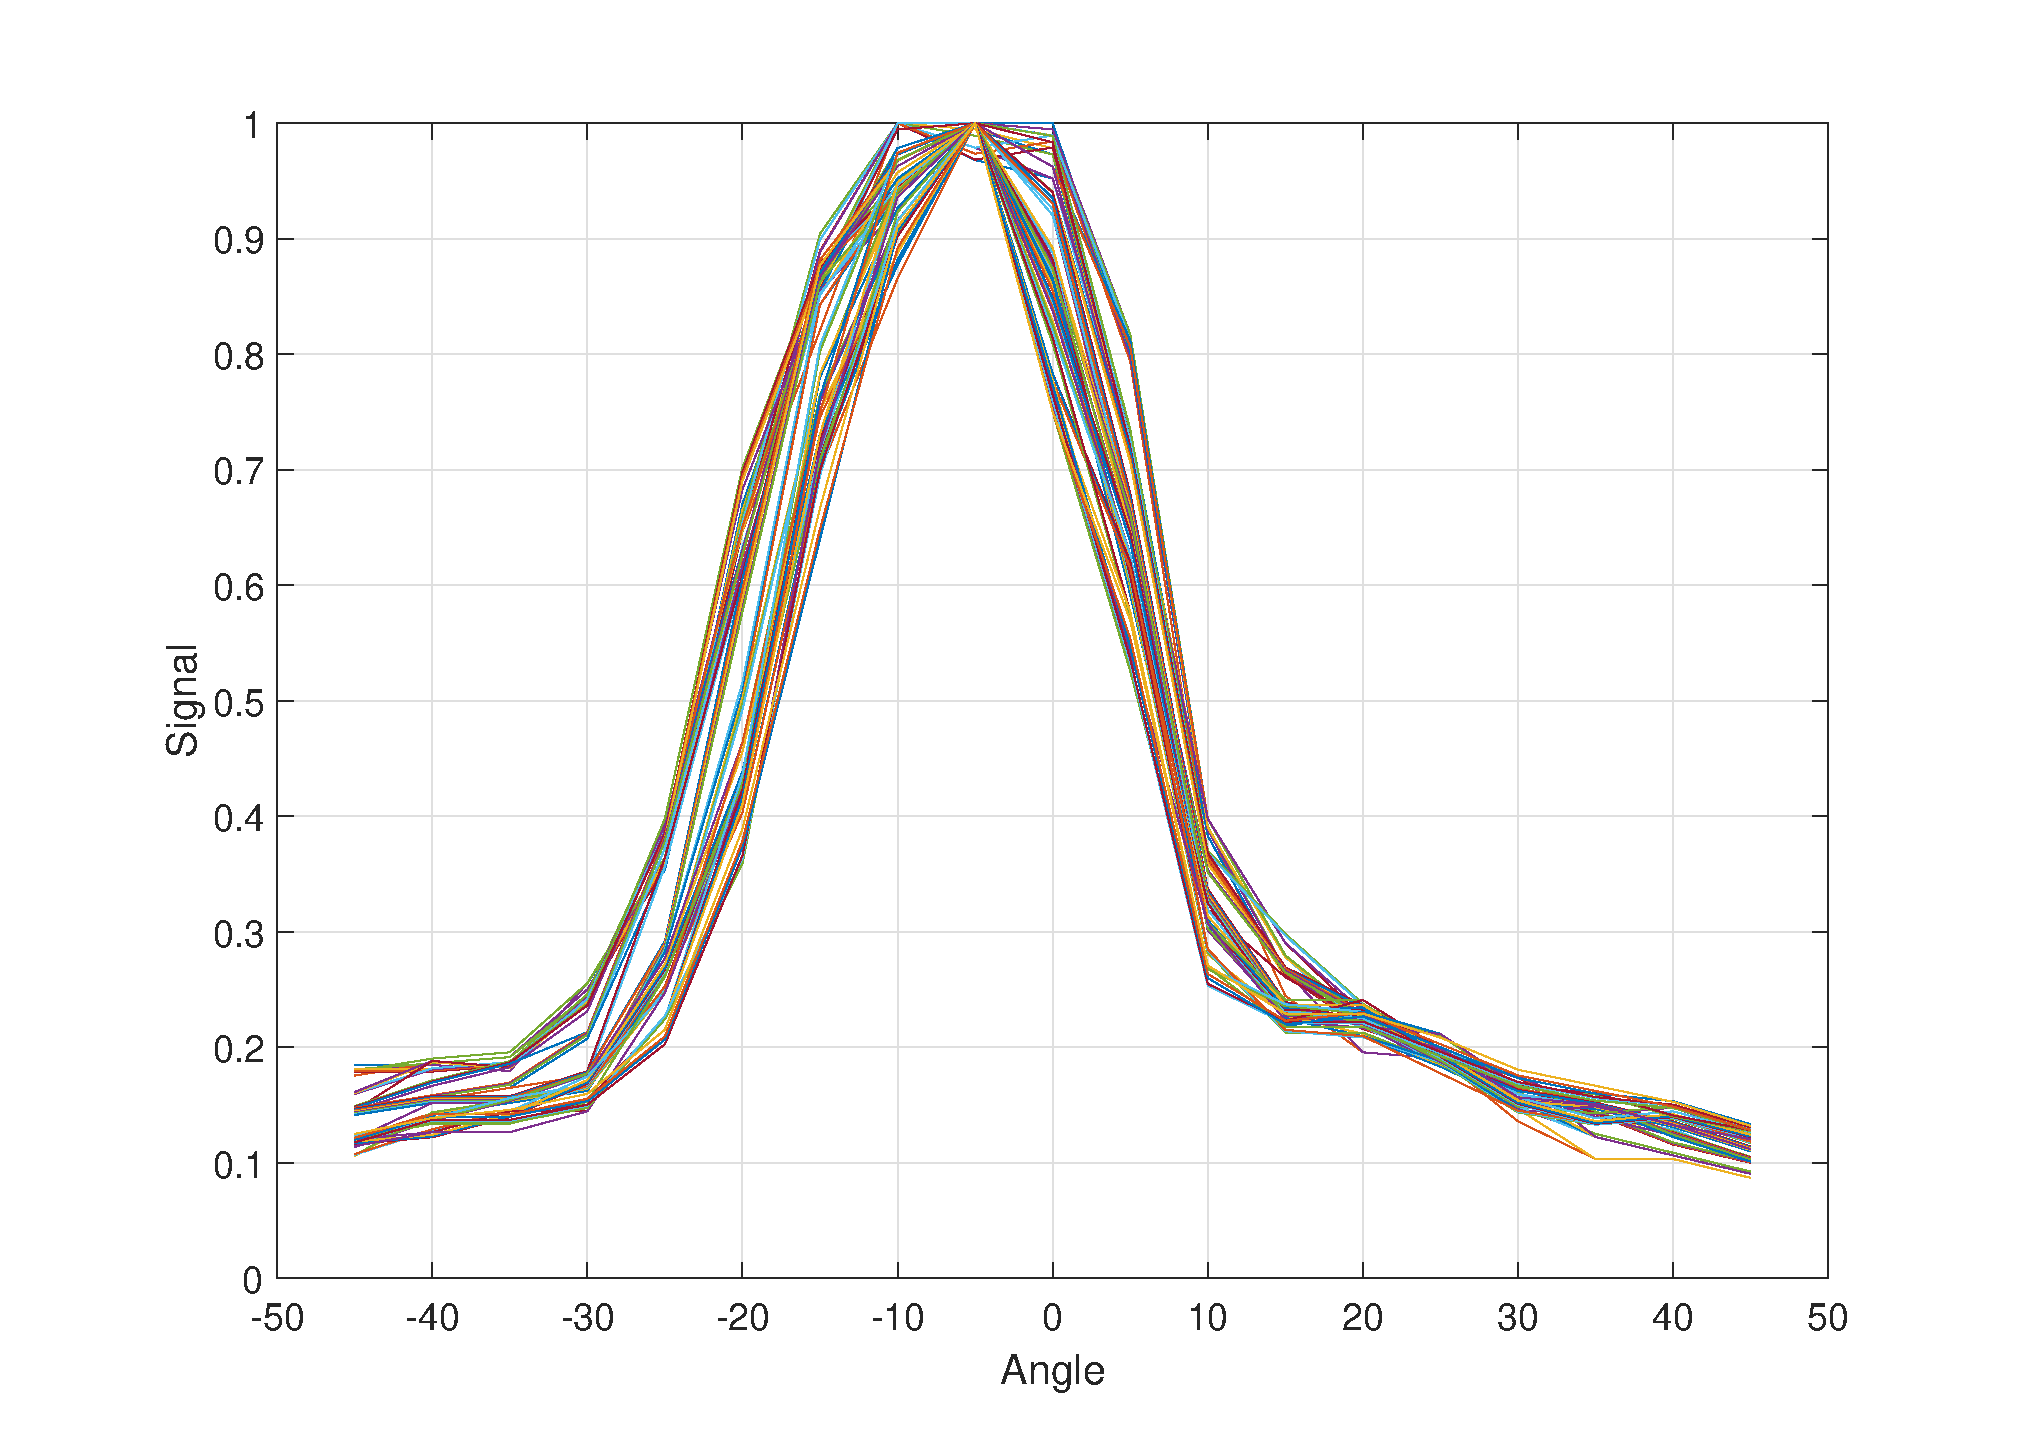
\includegraphics[width = 0.90\textwidth]{pics/ResponseXOffset}
\caption{Response for 100 different offset pixel positions from central diffraction pattern in X-direction}
\label{fig:offset_calib}
\end{figure}

\begin{figure}[!h]
\centering
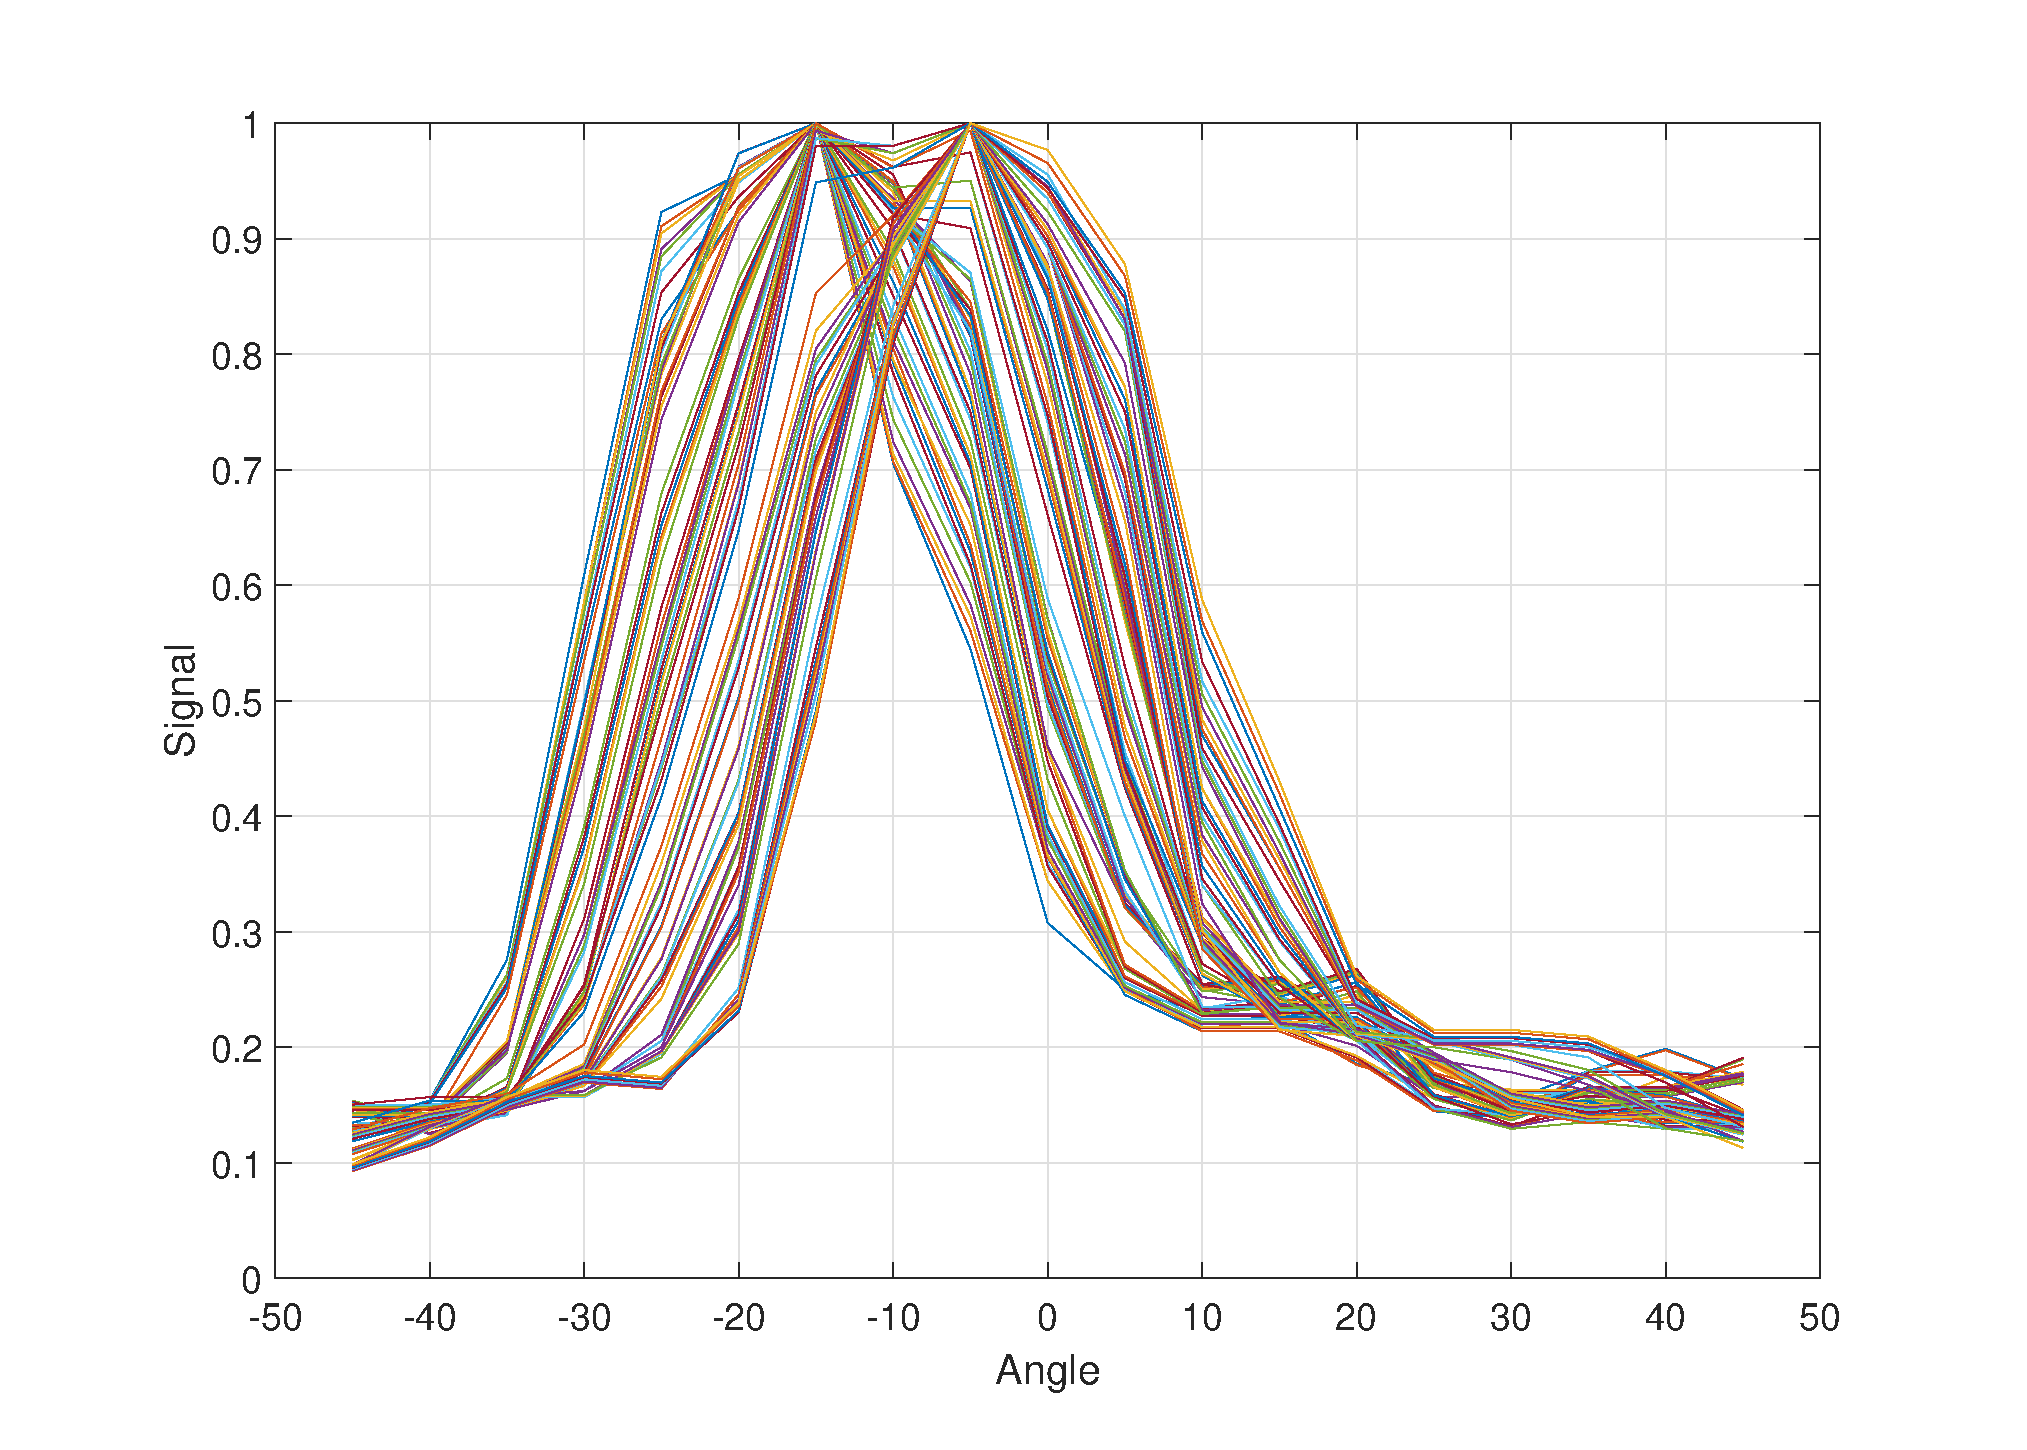
\includegraphics[width = 0.90\textwidth]{pics/ResponseYOffset}
\caption{Response for 100 different offset pixel positions from central diffraction pattern in Y-direction}
\label{fig:offset_calibY}
\end{figure}

The peak positions for different pixel offset positions in the X and Y direction is shown in \ref{fig:peak_pixel_pos}. It can be seen that pixels in the same neighborhood have the same peak angular positions. The shift in peak is seen as we move across the detector.  The peak angular position for different pixel positions is shown in Figure \ref{fig:peak_pixel_pos}.
This can be attributed to the non-uniformity in the laser beam that is used for measuring the response of the pixels.
\begin{figure}[!h]
\centering
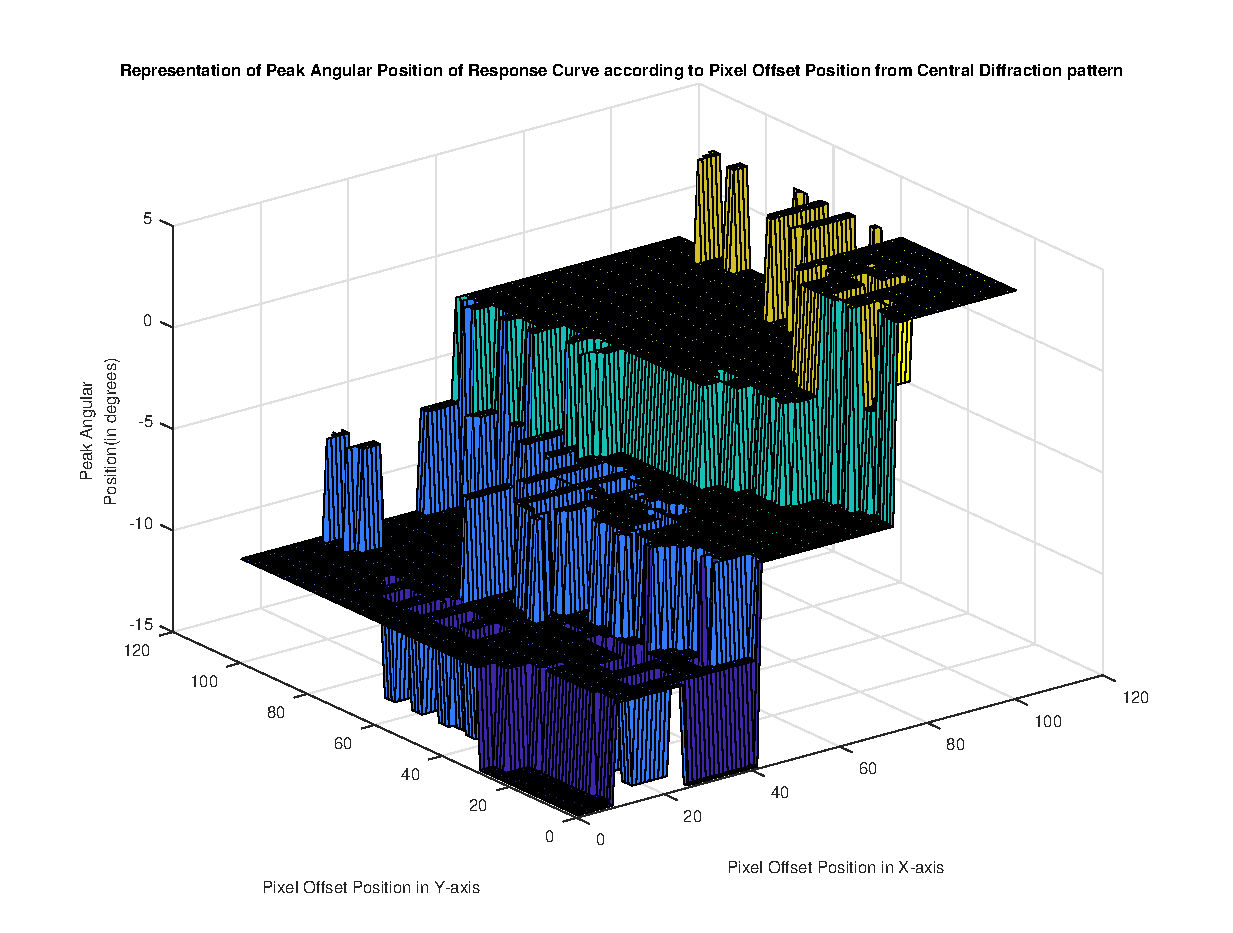
\includegraphics[width = \textwidth]{pics/MeshPlotAngularPeak}
\caption{Peak Angular Positions for different Pixels}
\label{fig:peak_pixel_pos}
\end{figure}

The experiment is repeated for 10 times and the response is plotted only for the red channel as we have only red frequency light hitting the sensor beam. The final result after solving the problems mentioned in the previous section is shown in Figure \ref{fig:acceptance_final}.
\begin{figure}[!h]
\centering
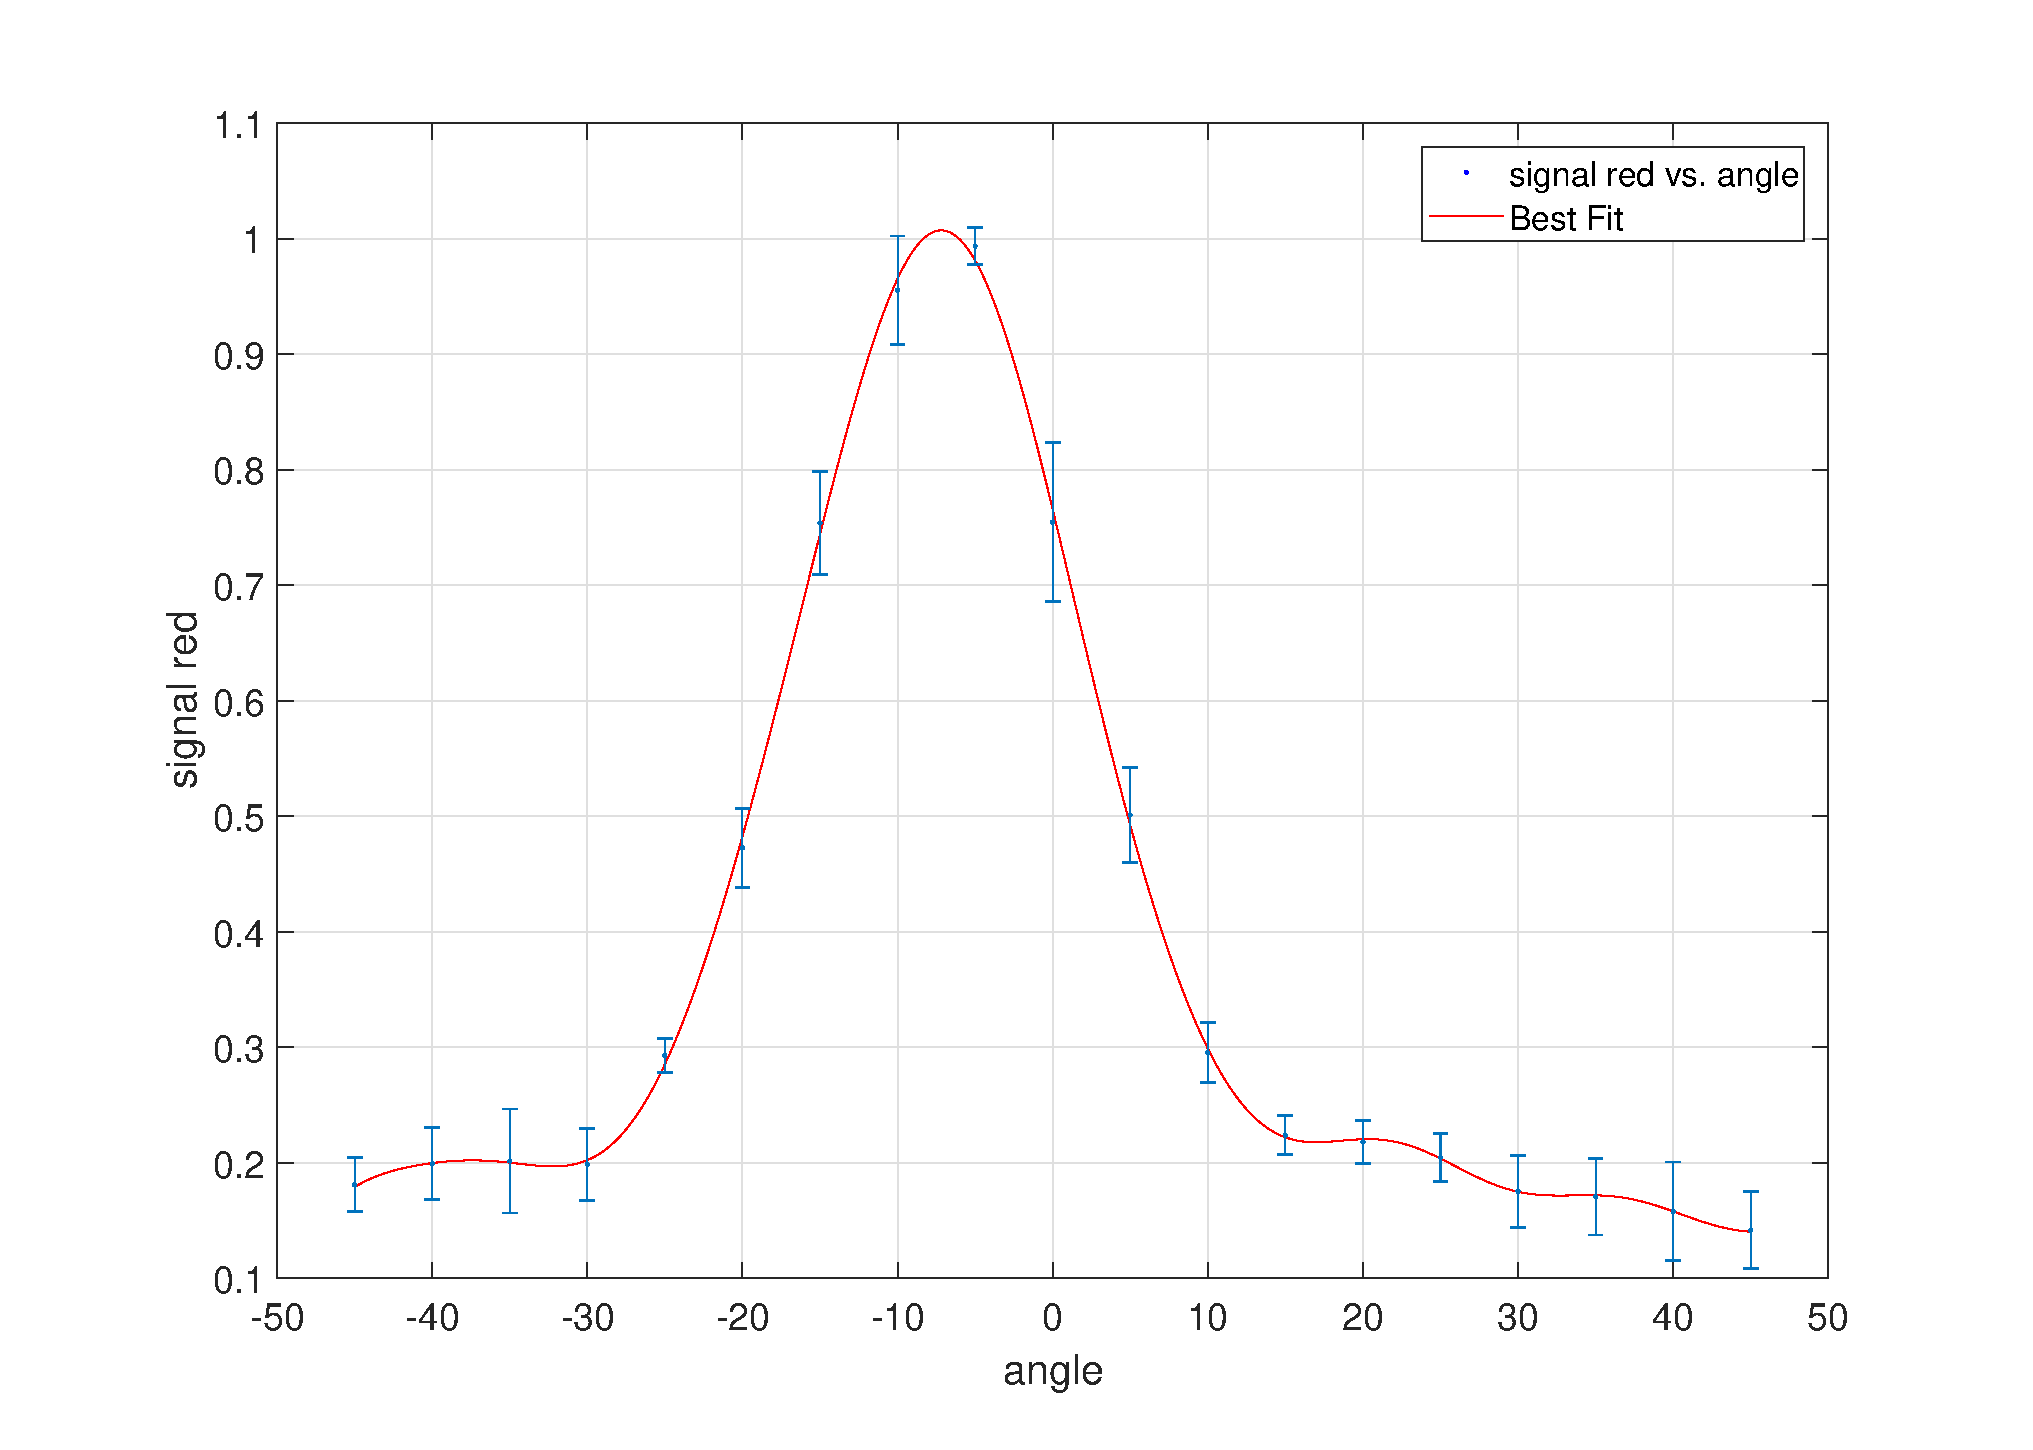
\includegraphics[width = \textwidth]{pics/FinalCRAExp}
\caption{Finalized Red Channel Response for Different Data Sets}
\label{fig:acceptance_final}
\end{figure}
There is less overlap in the subsequent angles and no points are excluded in the curve fitting process. The maximum standard deviation was reduced from 16 percent for the angular position -20(See Figure \ref{fig:exp_acc_red_1}) to 6 percent for angular position 0(See Figure \ref{fig:acceptance_final}). The peak of the curve is shifted towards -5$\degree$ because the maximum position of the laser beam occurs at -5$\degree$ position of the rotational beam. The graph data needs to be incorporated into the simulation to see the effect of the acceptance cone of the sensor on the image reconstruction. This will be discussed in the subsequent section.
\section{Adding to Simulation}
The curve data that was obtained in the previous experiment was incorporated into the previously obtained simulation results. In order to incorporate the data, we need to generate a 2-dimensional matrix that would simulate the behavior of the acceptance cone effect on the reconstruction. Since the behavior will be exhibited in both the horizontal and vertical directions, the 1-D curve was converted into 2-D by multiplying itself with its transpose. This would generate a circular symmetric matrix that would generate the effect of the acceptance cone in both the horizontal and vertical directions. This is shown in Figure \ref{fig:curve_sim}. We increase the effective interest area from $512 \times 512$ to $1024 \times 1024$ to visually see the number of pixels lost due to the acceptance angle effects. The mask size is changed accordingly to suit the image size.   
\begin{figure}[!h]
\centering
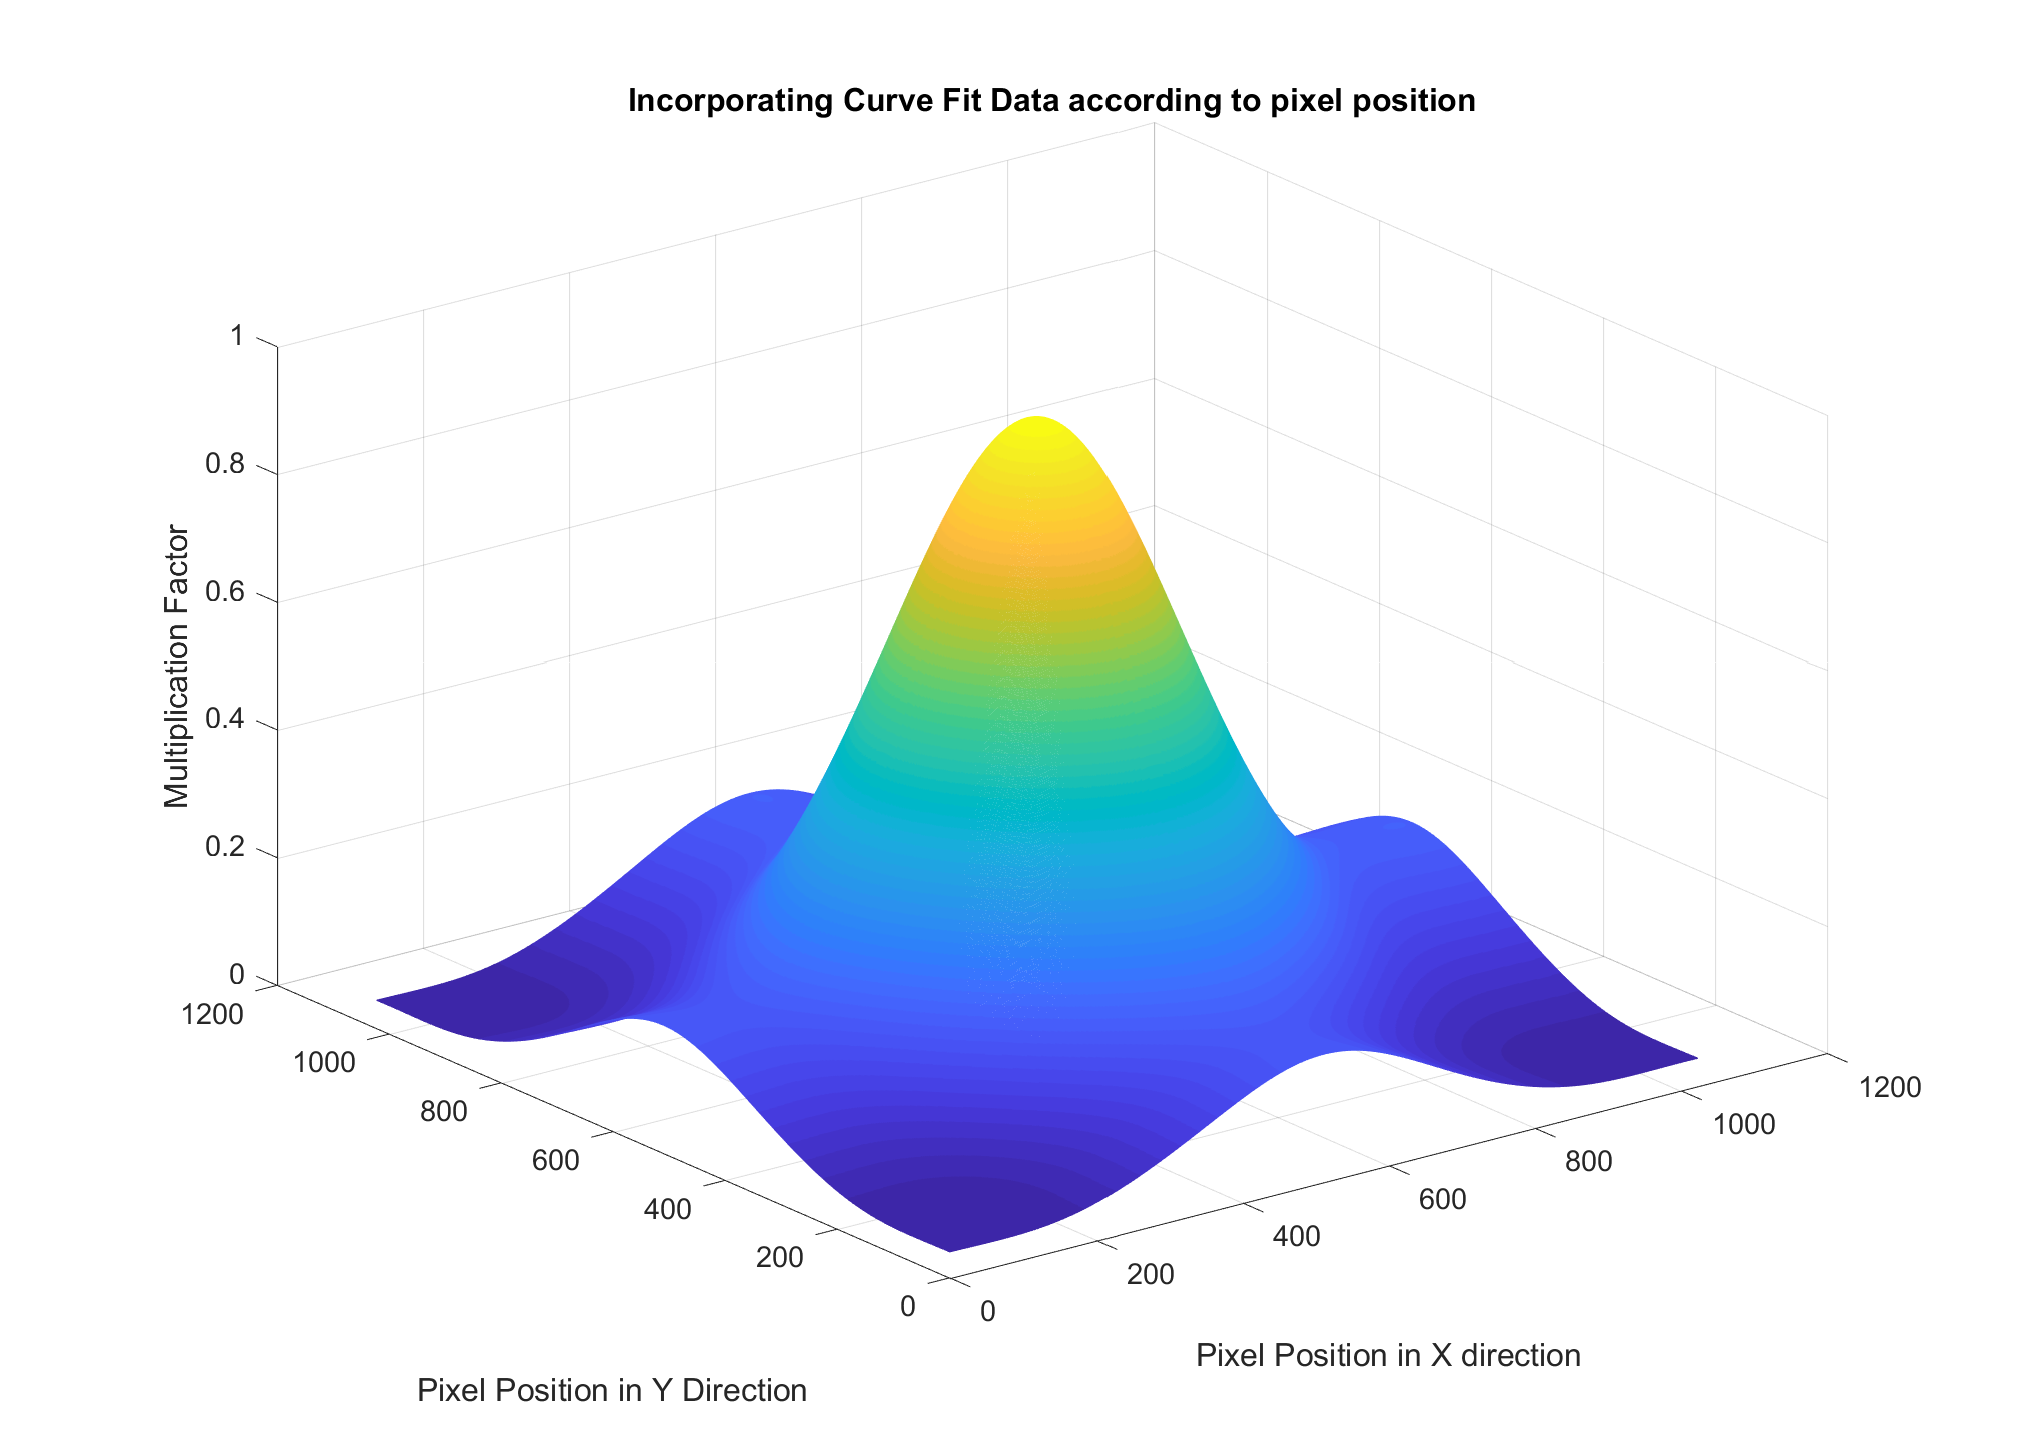
\includegraphics[width = \linewidth]{pics/AcceptanceConeCurveFit}
\caption{Fitted Curve Data into simulation}
\label{fig:curve_sim}
\end{figure}
This matrix is multiplied with the original image to simulate the effect of angle acceptance on the image reconstruction. This was tried with the simulation results that simulate the effects of diffraction to simulate as close to a real world. The source image, the reconstruction only with diffraction effects and the reconstruction with diffraction and acceptance cone is shown in Figure \ref{fig:rec_acc}. It can be seen that reconstruction with diffraction effects lead to a slight loss of detail. Once we incorporate the effects of acceptance cone into the simulation, it can be seen that only a portion of the original image can be reconstructed which is indicated by the square box in Figure \ref{fig:rec_acc}. 
This would be the actual field of view in the real world.  In order to find the angular field of view, the positions of the square box must be correlated with the fitted matrix curve discussed. On doing this, it can be found that the area in the rectangular box corresponds to an angle of -21.7$\degree$ to +21.7$\degree$. The angular field of view in absolute terms will be 43.4$\degree$ in the horizontal direction. The horizontal field of view and the vertical field of view can be considered to be equal since the pixel size of the CMOS sensor(OV2640) is the same in both directions.

 \begin{figure}[!h]
\centering
\includegraphics[width = \linewidth]{pics/ReconstructionAcce}
\caption{The image on the left indicates the original object image, the image in the middle indicates the reconstruction with only diffraction effects. The image on the right indicates both diffraction and acceptance angle effects. The red area indicates the effective amount of pixels that can be used. }
\label{fig:rec_acc}
\end{figure}
    

A lens based system would have a larger field of view depending on the lens used. The OV2640 camera module by default comes with a 1.4-inch lens with a field horizontal and vertical acceptance angle of $70\degree \times 63.7\degree$\cite{OV2640Arducam}\cite{lenses}. The lensless system would have a horizontal and vertical acceptance angle of view of $43.4\degree \times 43.4\degree$. This leads to a field of view reduction of 38 percent and 31.8 percent in the horizontal and vertical directions. The effective pixels that can be used by the camera is reduced to 48 percent meaning that only 48 percent of the total number of active pixels can be used for effective imaging. This is the trade-off that we need to face when we reduce the size of the camera by removing the lenses.

\section{Actual Field of View and Spatial Resolution Calculations}
In this section, we will be discussing how we can calculate the field of view of the camera from the experiment and will also perform spatial resolution calculations. This will give us an idea of how the camera will perform when used in an actual space application. The spatial resolution can be calculated using equation \ref{eq:spat_res_2}. 

\begin{equation}
\label{eq:spat_res_2}
d_s = \frac{d_p}{d_t} * d_h
\end{equation}

The calculated spatial resolutions($d_s$) based on mask-sensor distance($d_t$) and the height of the satellite($d_h$) from the earth is shown in Figure \ref{fig:spat-res-graph-1}. It can be seen from the graph that as we increase the mask-sensor distance, we can attain better spatial resolutions that can represent the ground data better. the best spatial resolution is obtained when the mask-sensor distance is the greatest(i.e 10 mm) and when the satellite is as close to the earth(350 kilometers). The best possible spatial resolution can be achieved at a height of 350 kilometers which would be 7.7 meters per pixel for a mask-sensor distance of 10 mm. A mask-sensor distance of 5 mm would provide 15.4 meters per pixel at the same height. It can be seen that if we make the camera thicker, we can get better spatial resolutions. The figure \ref{fig:spat-res-graph-1} is calculated for a pixel size of $2.2 \ \mu m \times 2.2 \ \mu m$. The other sensor OV5642 can offer a better spatial resolution as it's pixel size is smaller $1.4 \ \mu m \times 1.4 \ \mu m$. The spatial resolution values will be scaled by the ratio of the pixel sizes. 

\begin{figure}[]
\centering
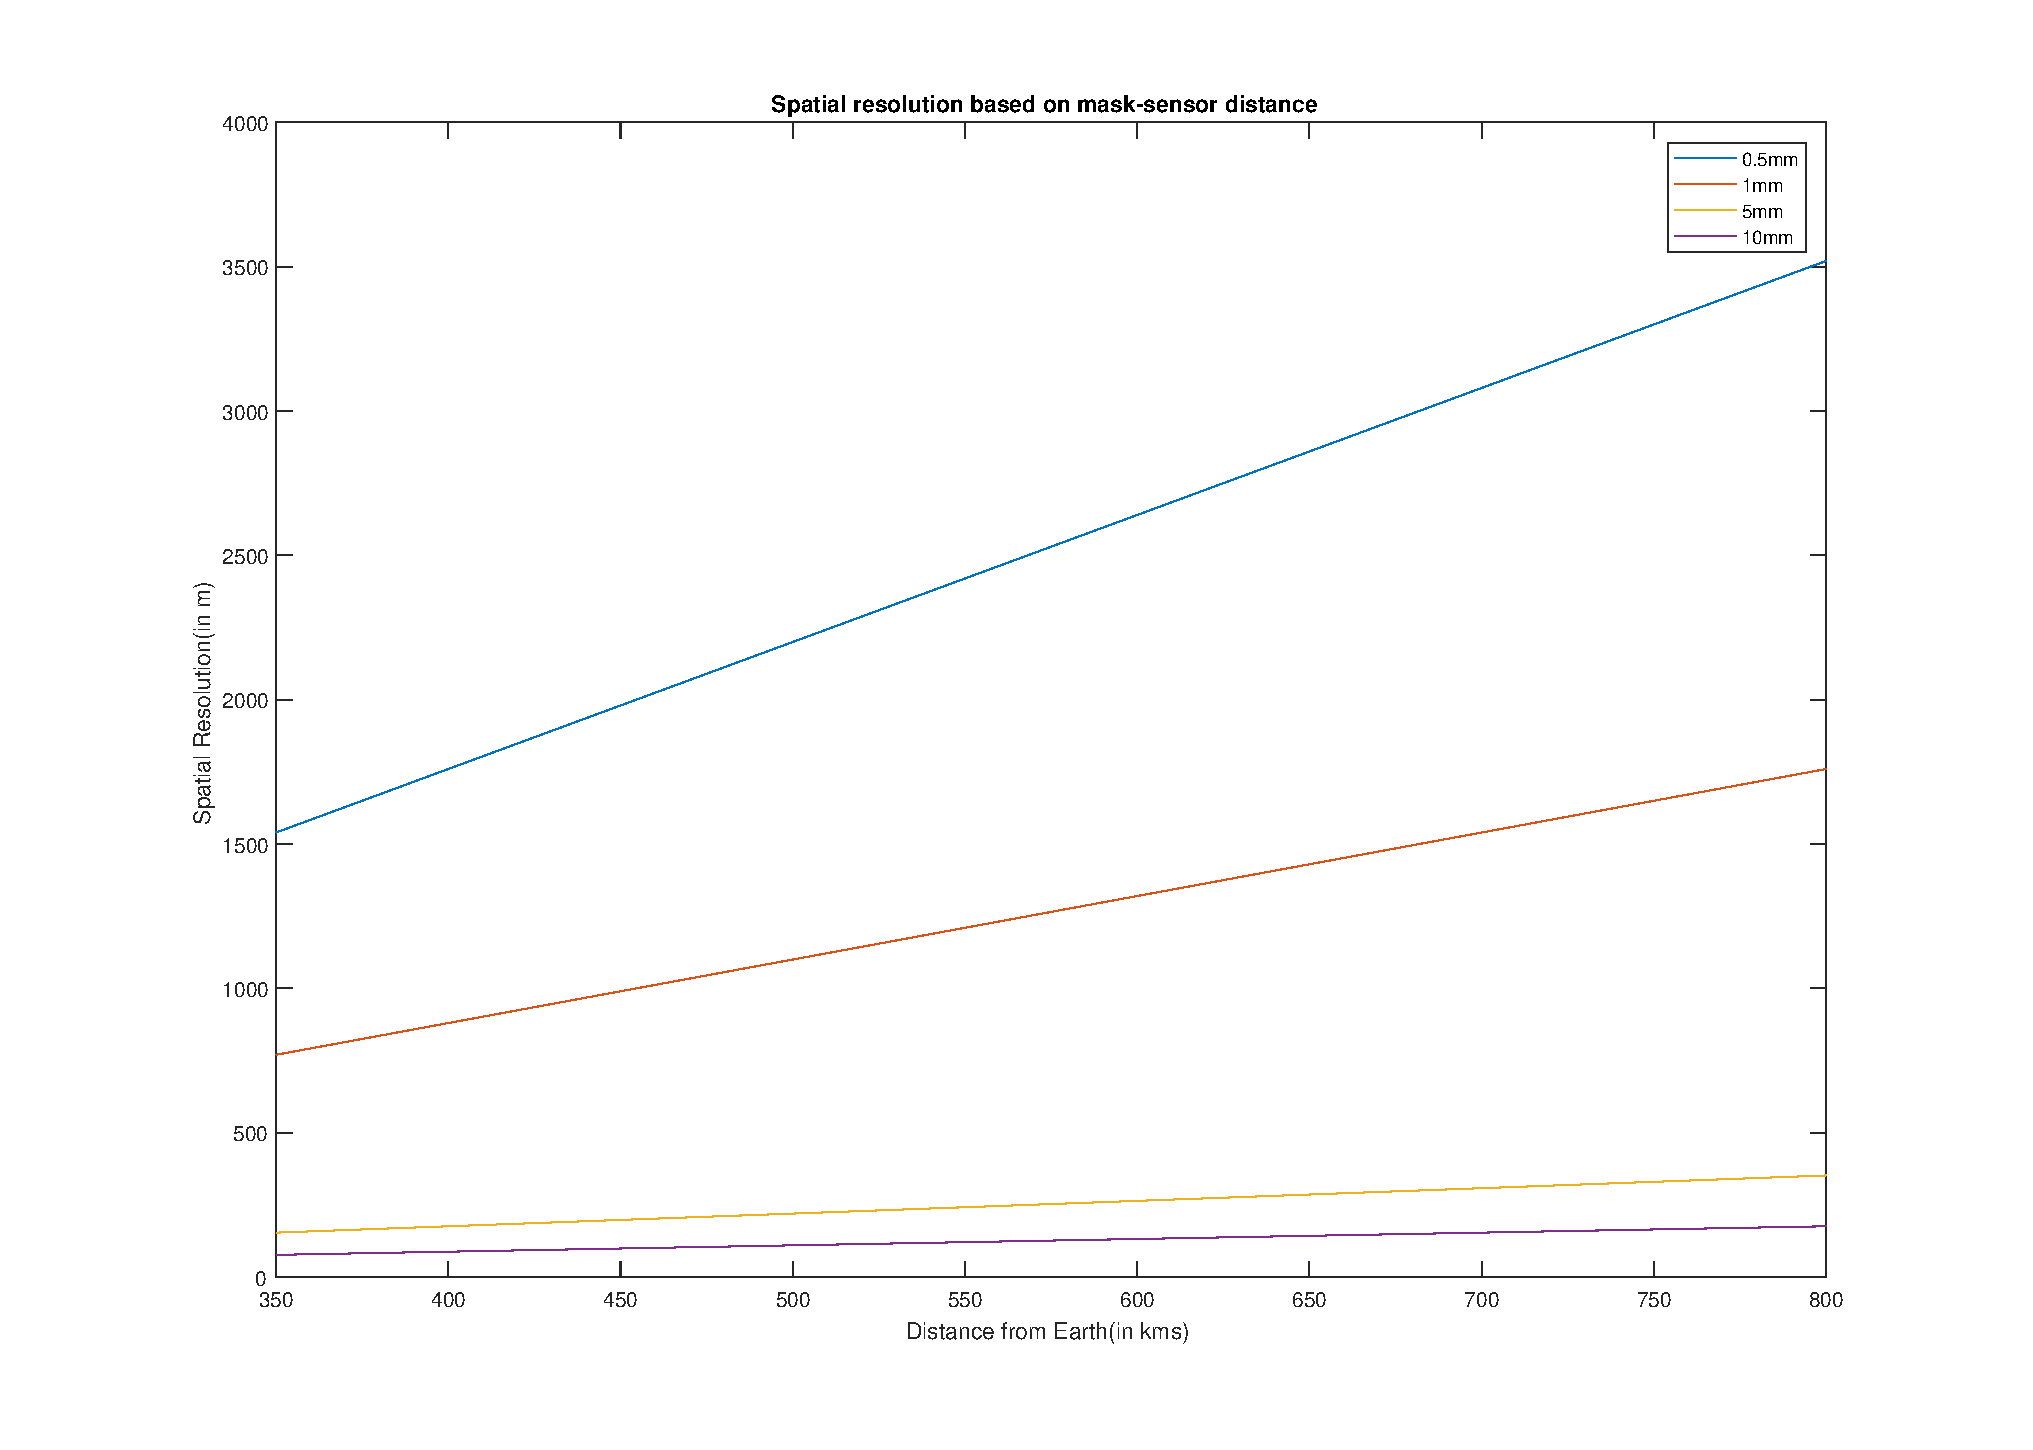
\includegraphics[width = \linewidth]{pics/spatial_res}
\caption{Relation between Spatial resolution and mask-sensor distance for sensor OV2640}
\label{fig:spat-res-graph-1}
\end{figure}

The field of view of the camera can be calculated using the acceptance angle calculated from integrating the experimental and simulation results. The sensor OV2640 has an experimentally verified acceptance angle of 21.7$\degree$($\theta_{cra}$). The field of view can be calculated using equation \ref{eq:fov_calc_2}. 
\begin{equation}
\label{eq:fov_calc_2}
d_{fov} = 2*d_h*tan(\theta_{cra})
\end{equation}
The obtained calculation results are shown in Figure \ref{fig:fov-graph-1}. It can be seen that maximum field of view can be obtained when the satellite is at a height of 800 kilometers from the surface of the earth. However, the spatial resolution as mentioned earlier will be lower at higher altitudes. A maximum field of view of 636 kilometers can be obtained at a height of 800 kilometers. The sensor OV5642 has an acceptance/chief ray angle of 23.6$\degree$ as mentioned in its data sheet\cite{OV5642DS}. However, this claim has not been experimentally verified.

\begin{figure}[]
\centering
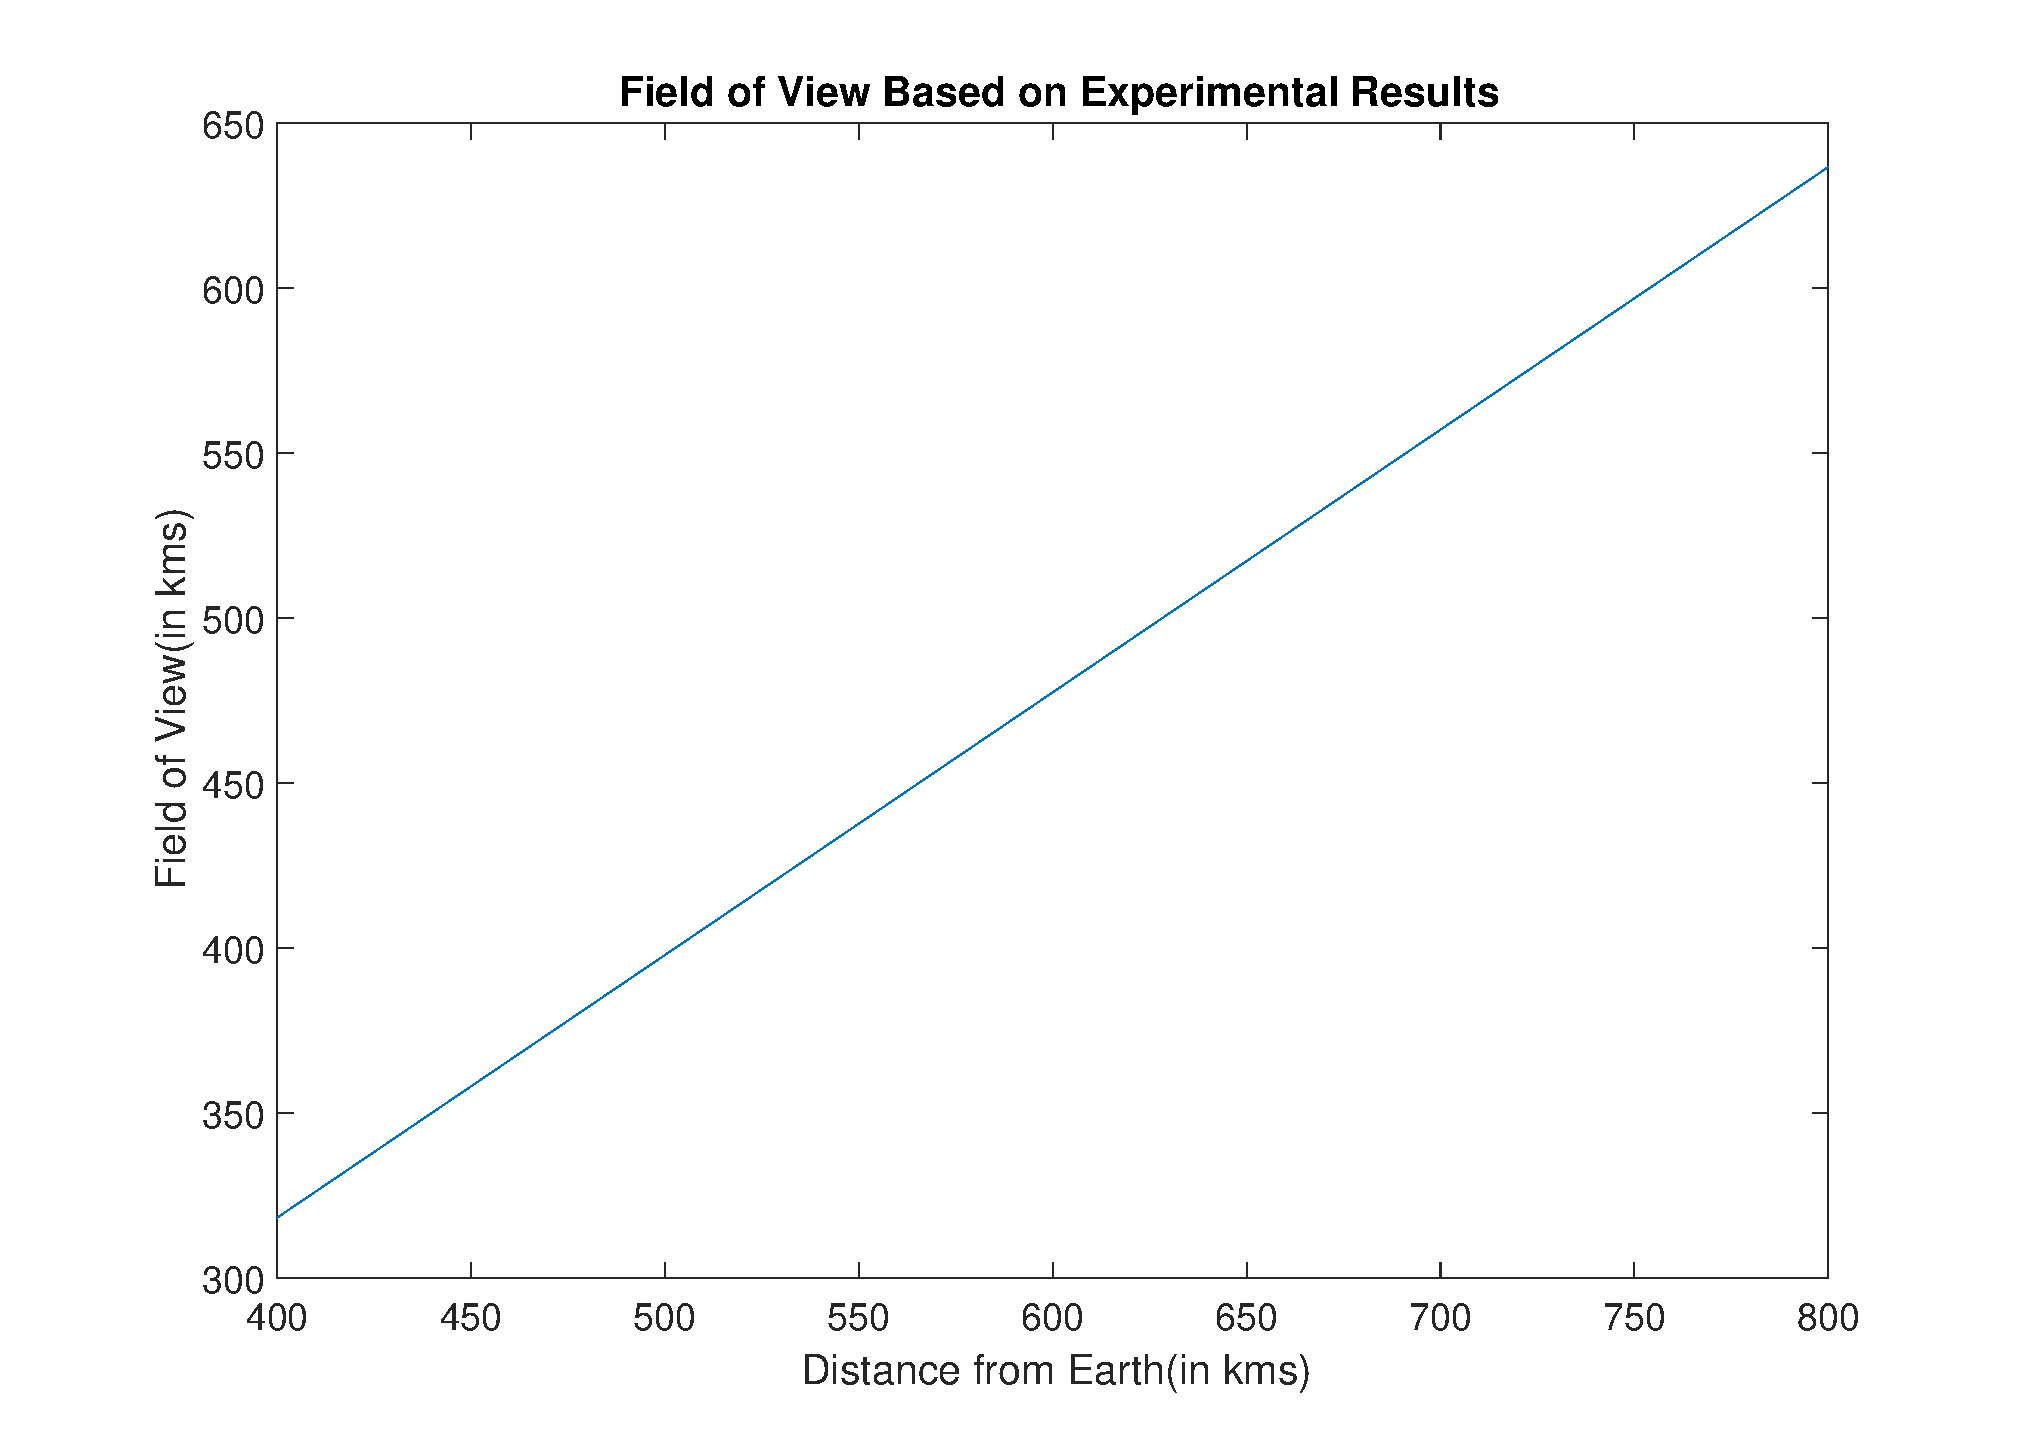
\includegraphics[width = \linewidth]{pics/FOV_Lensless}
\caption{Field of View Calculation based on Experimental Results}
\label{fig:fov-graph-1}
\end{figure}

\section{Spatial Light Modulators}
A spatial light modulator (SLM) is an object that imposes some form of spatially varying modulation on a beam of light\cite{SLMWiki}.SLMs can be controlled by computer controlled software and it would be possible to generate patterns on the SLM that could modulate phase or the intensity of the beam or both simultaneously. An advantage of using an SLM over designing a lithographic mask is that it would be possible to test out different designs of masks quickly in order to find out an optimal mask configuration that would be suitable to our setup. In our design of the lensless imager, it must be possible to block and allow light in a certain binary pattern. A transmissive SLM would suit the purpose of simulating different mask patterns. For this purpose, a Holoeye LC2012 SLM was used. The SLM has a pixel area of $1024 \times 768$ and a pixel pitch of $36\  \mu m$.

\begin{figure}[ht]
\centering
\includegraphics[width=0.50\textwidth]{pics/slm}
\caption{HoloEye LC2012 SLM}
\label{fig:slm}
\end{figure}

% CONCLUSIONS AND FUTURE WORK
\chapter{Conclusions and Future Work}
\label{chp:conclusionsandfuturework}

\section{Goals and Research Questions revisited}
In the beginning of the chapter, a research question and goals for the project were proposed. Now, let us revisit them to find out whether we have reached the goals of the project. The project was divided into these four sub-questions as given below:
\begin{itemize}
\item What would be the image sensor that can be used for the camera? \\
In chapter 2 of this report, a survey of image sensors is conducted and the drawbacks of each sensor are presented. Based on various factors, OV2640 and OV5642 were chosen. This also indicates the achievement of the first goal.
\item How do we design the hardware and software for such a camera that can be used in Delfi-PQ satellite?\\
The main factor in choosing OV2640 and OV5642 was the presence of open source libraries,  and open source electronic interface hardware. The software and the hardware mechanism for controlling the cameras have been described in Chapter 4 of the report. All the experiments described in the later chapters of the report were developed using the same hardware and software described in Chapter 4. This also indicates the achievement of the second goal.
\item What would be the field of view and spatial resolution of the lensless camera?\\
An experimental setup to determine the acceptance cone of the image sensor has been devised. The experimental results were incorporated into the previously completed simulations. Based on the experimental results, OV2640 had an acceptance angle of 43.6 degrees. It was found that the field of view of the lensless system had reduced 38 percent and 31.8 percent in the horizontal and vertical directions compared to a conventional lens based system. The effective area of the sensor that could be used also reduced by 52 percent. The spatial resolution of the designed camera was calculated and the entire procedure for calculating the spatial resolution is described in Chapter 2 and Chapter 5 of the report. This also indicates the achievement of the third goal. The experiments for finding out the acceptance angle was performed using the OV2640. The OV5642 has an acceptance angle of 23 degrees(given by the datasheet). However, this claim is yet to be verified experimentally.
\item What would be the computational algorithm that would be used in such a lensless camera? \\
The computational algorithm mainly depends on the mask that we use for imaging. Doubly Toeplitz masks were chosen since they retain the separable property even in the presence of diffraction. The computational reconstruction method for separable doubly Toeplitz mask has been studied and simulated. It was found in the simulations that separable doubly Toeplitz mask could be used to reconstruct objects even in the presence of diffraction effects. The entire simulation workflow is described in Chapter 3 of the report.

\item How do we experimentally prove the concept of lensless imaging? \\
Experimental verification of lensless imaging required multiple stages of experiments. After determining the field of view of the OV2640 sensor, the imaging of the separable mask was tried using OV2640. However, it was found out that OV2640 could not be used due to the limitation of the onboard FIFO buffer of the camera. Because of this, we decided to use OV5642 which has a bigger FIFO buffer. OV5642 is able to image the mask perfectly and preserves the separable property of the mask. The entire experimental approach was done using singular value decomposition and is mentioned in Chapter 6 of the report.  

The next step was to determine the system matrices of the lensless camera. To do this, we decide to use a Hadamard basis matrix as it could provide enough amount of light to produce a measurable sensor response. Using a basis matrix also provided better reconstruction and preserved the original object property as seen in the simulation results. This method requires us to use $2N$ calibration patterns on the LCD if we want to reconstruct images of resolution $N \times N$. This method was not verified experimentally and forms the final step of proving the concept of lensless imaging experimentally. The strategy and scheme for achieving this are described in Chapter 7 of the report. This indicates that there is some more experimental verification required to achieve the final goal.

\end{itemize}

Now, let us come to the main research question:
\textbf{Is it possible to design ``lensless coded aperture" cameras with a small form-factor(thickness $<=$ 10 mm) using COTS(commercially available off-the-shelf) components that can be used in U-class Spacecraft ?}\\
The experimental results with commercially available camera modules OV2640 and OV5642 provide a good insight into the lensless imaging methodologies. The previous studies done in this field did not have any memory limitations like we faced with OV2640. The camera with bigger memory such as OV5642 could retain the properties of the mask when we experimentally tested them. A separable scene on the outside also yields a separable scene on the image sensor. A scheme for determining the system matrices of a lensless imaging system is designed and simulated. However, the experimental determination of this scheme has not yet been verified. The simulations and experiments done in this work provide a good picture and insight into the concept of lensless imaging as a whole. The experimental results achieved till now indicate that commercially available cameras can be used but more experiments need to be performed before this question can be answered with more certainty. 

\section{Future Work}
With the developed calibration patterns, it would be possible to reconstruct images of resolution $N \times N$. $N$ should be a power of 2 since the Hadamard basis matrices can only be generated as a square matrix whose rows and columns have sizes which are a power of 2. With the OV2640(currently not usable due to memory limitations) and OV5642, a maximum possible image of resolution $1024 \times 1024$, can be reconstructed if we are able to estimate the system matrices using these sensors experimentally. OV2640 consumes approximately 465 mW for a full-resolution picture(1600 $\times$ 1200) and OV5642 consumes 1.165 W for a full-resolution picture(2592 $\times$ 1944). The Delfi-PQ team has allotted a 4W budget for the entire imager(including the microcontroller). If OV5642 is chosen, 2.8W will remain for the microcontroller and the RS-485 data interface circuitry which would be used for communication with the main onboard computer of the satellite. At this stage, it would not be possible to decide the exact thickness of the camera as the final-proof-of-concept is not yet available.

It was observed during the experiments that the sensor was not able to produce an output in correlation with the simulation data. The problem was traced to the non-binary behavior of the mask produced by SLM. A fabricated photomask can provide us with superior performance compared to an SLM. It would be possible to stick the photomask to the glass plate on the sensor(which leads to a thickness of $500 \ \mu m$ ). With the current setup, it was not possible to bring the sensor closer than 1 centimeter. There is a great scope for developing the work mentioned in this thesis. This work can be improved and extended in the following ways:
\begin{itemize}
\item Experimental determination of System Matrices: A scheme for experimental determination of the system matrix has been described in Chapter 7 of the report. This needs to be completed to completely realize the concept of lensless imaging. The scheme described is extremely time-consuming as it requires $2N$ measurements(one-time procedure) to perform complete reconstructions for $N \times N$ resolution images. This scheme can also be improved to reduce the number of measurements needed to accurately estimate the system matrices. 

\item Fabrication with masks: This work uses transmissive Spatial light modulators(SLM) to simulate the effects of a mask. It was observed that a complete binary mask cannot be achieved with this equipment. Lithographic photomasks can be fabricated and can offer better performance than using an SLM. The system matrices must also be estimated for a photomask based lensless imaging system.

\item Improving the computational method for reconstruction: This work uses regularization along with matrix inversion to perform reconstructions. This method can also be improved using other methods to denoise the reconstruction such as SVD, BM3D and total variation based methods\cite{Flatcam}. These methods could be tried out on the existing simulations and studied whether they provide better reconstructions.

\item Hardware Improvements: OV2640 could not be used due to the limited onboard memory. The future work can also look into improving the camera hardware by replacing the memory of the camera module. This would also require a change in the hardware/software implementations of the library. Arducam can be contacted on how to achieve this. Also, they release improved versions of the camera modules every year.
\end{itemize}



% BIBLIOGRAPHY
%#define SORTED 1
\bibliographystyle{../bib/latex8}
\bibliography{../bib/mycollection}

%\appendix

%\chapter*{Appendix}
\addcontentsline{toc}{chapter}{Appendix}
\section*{Fresnel Propagation Model}
In this section, we will briefly discuss the Fresnel propagation model used for obtaining the effects of diffraction. The model is based on \cite{FourierOptics} and the MATLAB model developed at Optica Group was used. When modeling the diffraction effect, we have a source plane and an observation plane. In our case, the source plane is the mask and the observation plane would be the sensor. This is shown in Figure \ref{fig:fresnel_1}. 
\begin{figure}[!htbp]
\centering
\includegraphics[width = \linewidth]{pics/fresnel-1}
\caption{Source Plane and Observation Plane}
\label{fig:fresnel_1}
\end{figure}
The diffraction effects lie in the Fresnel region since the Fresnel number would be less than one. In this case, the diffraction effects can be given by the equation \ref{eq:fresnel-1}.

\begin{equation}
\label{eq:fresnel-1}
U_2(x,y) = \frac{e^{jkz}}{j\lambda z}\int \int U_1(\xi, \eta )exp(\frac{jk}{2z}[(x - \xi)^2 + (y - \eta)^2])d\xi d\eta
\end{equation}
This expression can also be written in the form of equation \ref{eq:fresnel-2}.
\begin{equation}
\label{eq:fresnel-2}
U_2(x,y) = F^{-1}(F(U_1(x,y)F(h(x,y)))
\end{equation}
where
\begin{equation}
\label{eq:fresnel-3}
h(x,y) = \frac{e^{jkz}}{j\lambda z}exp(\frac{jk}{2z}(x^2 + y^2))
\end{equation}

\section*{Appendix A Camera Dimensions}
This section shows the dimension of the camera module as provided by the camera vendor.

\begin{figure}[!htbp]
\centering
\includegraphics[width = 0.75 \linewidth]{pics/arducam_mech}
\caption{Dimensions of both OV5642 and OV2640 camera modules}
\label{fig:arducam_mech}
\end{figure}



\end{document}

